\documentclass[supercite]{Experimental_Report}

\title{~~~~~~数据结构实验~~~~~~}
\author{徐越扬}
\school{计算机科学与技术学院}
\classnum{CS2410}
\stunum{U202414825}
\instructor{郑渤龙} 
\date{2022年6月12日}

\usepackage{algorithm, multirow}
\usepackage{algpseudocode}
\usepackage{amsmath}
\usepackage{amsthm}
\usepackage{framed}
\usepackage{mathtools}
\usepackage{subcaption}
\usepackage{xltxtra} %提供了针对XeTeX的改进并且加入了XeTeX的LOGO, 自动调用xunicode宏包(提供Unicode字符宏)
\usepackage{bm}
\usepackage{tikz}
\usepackage{tikzscale}
\usepackage{pgfplots}
\usepackage{listings}
\usepackage{xcolor}
\usepackage{pifont}
%\usepackage{enumerate}

\pgfplotsset{compat=1.16}

\newcommand{\cfig}[3]{
  \begin{figure}[htb]
    \centering
    \includegraphics[width=#2\textwidth]{images/#1.tikz}
    \caption{#3}
   \label{fig:#1}
  \end{figure}
}

\newcommand{\sfig}[3]{
  \begin{subfigure}[b]{#2\textwidth}
    \includegraphics[width=\textwidth]{images/#1.tikz}
    \caption{#3}
   \label{fig:#1}
  \end{subfigure}
}

\newcommand{\xfig}[3]{
  \begin{figure}[htb]
    \centering
    #3
    \caption{#2}
    \label{fig:#1}
  \end{figure}
}

\lstset{
basicstyle=\small,                 % 设置整体的字体大小
frame=lines,                               % 设置代码块边框
showstringspaces=false,                % 不显示字符串中的空格
numbers=left,                               % 在左侧显示行号
breaklines=true,                           %对过长的代码自动换行
% numberstyle=\scriptsize\color{gray},    % 设置行号格式
%numberstyle=\color{darkgray},               % 设置行号格式
backgroundcolor=\color{white},              % 设置背景颜色
keywordstyle=\color{blue},                  % 设置关键字颜色
commentstyle=\it\color[RGB]{0,100,0},       % 设置代码注释的格式
stringstyle=\sl\color{red},                 % 设置字符串格式
xleftmargin = 2em,
%xrigntmargin = 2em,
}

\newcommand{\whiteding}[1]{\ding{\numexpr171+#1\relax}}

\newcommand{\rfig}[1]{\autoref{fig:#1}}
\newcommand{\ralg}[1]{\autoref{alg:#1}}
\newcommand{\rthm}[1]{\autoref{thm:#1}}
\newcommand{\rlem}[1]{\autoref{lem:#1}}
\newcommand{\reqn}[1]{\autoref{eqn:#1}}
\newcommand{\rtbl}[1]{\autoref{tbl:#1}}

\algnewcommand\Null{\textsc{null }}
\algnewcommand\algorithmicinput{\textbf{Input:}}
\algnewcommand\Input{\item[\algorithmicinput]}
\algnewcommand\algorithmicoutput{\textbf{Output:}}
\algnewcommand\Output{\item[\algorithmicoutput]}
\algnewcommand\algorithmicbreak{\textbf{break}}
\algnewcommand\Break{\algorithmicbreak}
\algnewcommand\algorithmiccontinue{\textbf{continue}}
\algnewcommand\Continue{\algorithmiccontinue}
\algnewcommand{\LeftCom}[1]{\State $\triangleright$ #1}

\newtheorem{thm}{定理}[section]
\newtheorem{lem}{引理}[section]

\colorlet{shadecolor}{black!15}

\theoremstyle{definition}
\newtheorem{alg}{算法}[section]

\def\thmautorefname~#1\null{定理~#1~\null}
\def\lemautorefname~#1\null{引理~#1~\null}
\def\algautorefname~#1\null{算法~#1~\null}

\begin{document}

\maketitle

\clearpage

\pagenumbering{Roman}

\tableofcontents[level=2]

\clearpage

\pagenumbering{arabic}

\section{基于顺序存储结构的线性表实现}

\subsection{问题描述}

线性表(Linear List)是最基本、最常用的一种数据结构,用来存储具有线性关系的一组数据元素。它是具有相同数据类型的n个数据元素的有限序列,每个元素有唯一的前驱和后继(第一个元素除外没有前驱,最后一个元素除外没有后继)。线性表有两种主要的存储方式:顺序存储结构(数组),链式存储结构(链表)。前者是把线性表的元素存储在一块连续的内存空间中,而后者包含每个元素的存储数据和指向下一个元素的指针。在优缺点方面:前者可以快速随机的访问元素,但是插入删除效率较低。后者插入删除效率高,但是必须从头访问。不同的情形下两者的使用不同。

本实验要求构造一个具有菜单的功能演示系统。其中,在主程序中完成函数调用所需实参值的准备以及执行结果的显示,并给出正确的操作提示。该程序实现了线性表的初始化、销毁线性表、清空线性表、线性表判空、求线性表表长、获得元素等基本功能,以及最大连续子数组和、和为K的子数组、顺序表排序等附加功能。可以以文件的形式进行存储和加载。同时实现多线性表管理,完成多线性表的添加、删除、定位,查找和展示等操作。

\subsection{系统设计}

\subsubsection{头文件和预定义}

1、头文件

\begin{lstlisting}[language=c]
#include <stdio.h>
#include <malloc.h>
#include <stdlib.h>
#include <string.h>
\end{lstlisting}

2、预定义常量

\begin{lstlisting}[language=c]
#define TRUE 1
#define FALSE 0
#define OK 1
#define ERROR 0
#define INFEASIBLE -1
#define OVERFLOW -2
#define LIST_INIT_SIZE 100
#define LISTINCREMENT  10
\end{lstlisting}

3、类型表达式

\begin{lstlisting}[language=c]
typedef int status;
typedef int ElemType; //数据元素类型定义
typedef struct{  //顺序表的定义
    ElemType * elem;
    int length;
    int listsize;
}SqList;
typedef struct{  //线性表的集合类型定义
    struct { 
        char name[30];
        SqList L;
    } elem[10];
    int length;
    int listsize;
}LISTS;
\end{lstlisting}

\subsubsection{基本功能函数}

 \begin{figure}[H]
 	\centering
 	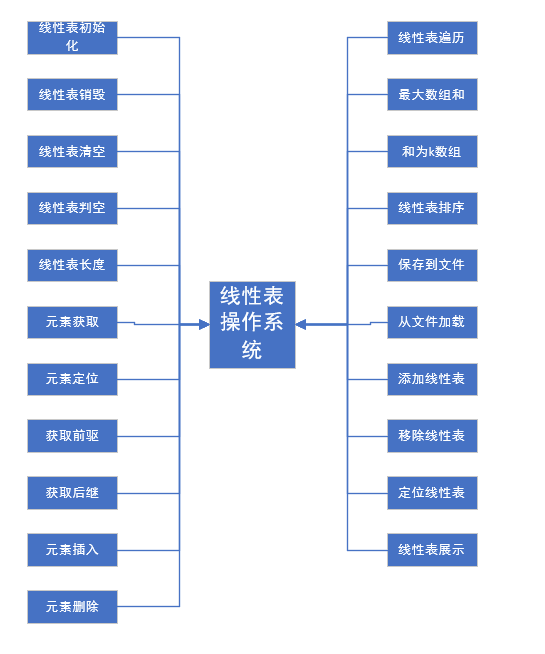
\includegraphics[width=0.9\textwidth]{images/系统概图.png}
 	\caption{系统整体功能图}
 	\label{txlab}
 \end{figure}

依据最小完备性和常用性相结合的原则,以函数形式定义了线性表的初始化表、销毁表、清空表、判定空表、求表长和获得元素等12种基本运算,具体运算功能定义如下:

\begin{enumerate}
    \item 初始化表:函数名称是InitList(L);初始条件是线性表L不存在;操作结果是构造一个空的线性表;
    \item 销毁表:函数名称是DestroyList(L);初始条件是线性表L已存在;操作结果是销毁线性表L;
    \item 清空表:函数名称是ClearList(L);初始条件是线性表L已存在;操作结果是将L重置为空表;
    \item 判定空表:函数名称是ListEmpty(L);初始条件是线性表L已存在;操作结果是若L为空表则返回TRUE,否则返回FALSE;
    \item 求表长:函数名称是ListLength(L);初始条件是线性表已存在;操作结果是返回L中数据元素的个数;
    \item 获得元素:函数名称是GetElem(L,i,e);初始条件是线性表已存在,同时需要满足1≤i≤ListLength(L);操作结果是用e返回L中第i个数据元素的值;
    \item 查找元素:函数名称是LocateElem(L,e,compare());初始条件是线性表已存在;操作结果是返回L中第1个与e满足关系compare()关系的数据元素的位序,若这样的数据元素不存在,则返回值为0;
	\item 获得前驱:函数名称是PriorElem(L,cur\_e,pre\_e);初始条件是线性表L已存在;操作结果是若cur\_e是L的数据元素,且不是第一个,则用pre\_e返回它的前驱,否则操作失败,pre\_e无定义;
	\item 获得后继:函数名称是NextElem(L,cur\_e,next\_e);初始条件是线性表L已存在;操作结果是若cur\_e是L的数据元素,且不是最后一个,则用next\_e返回它的后继,否则操作失败,next\_e无定义;
	\item 插入元素:函数名称是ListInsert(L,i,e);初始条件是线性表L已存在,同时需要满足1≤i≤ListLength(L)+1;操作结果是在L的第i个位置之前插入新的数据元素e。
	\item 删除元素:函数名称是ListDelete(L,i,e);初始条件是线性表L已存在且非空,1≤i≤ListLength(L);操作结果:删除L的第i个数据元素,用e返回其值;
	\item 遍历表:函数名称是ListTraverse(L,visit()),初始条件是线性表L已存在;操作结果是依次对L的每个数据元素调用函数visit()。
\end{enumerate}

\subsubsection{附加功能函数}

\begin{enumerate}
    \item 最大连续子数组和:函数名称是MaxSubArray(L); 初始条件是线性表L已存在且非空,请找出一个具有最大和的连续子数组(子数组最少包含一个元素),操作结果是其最大和;
    \item 和为K的子数组:函数名称是SubArrayNum(L,k); 初始条件是线性表L已存在且非空, 操作结果是该数组中和为k的连续子数组的个数;
    \item 顺序表排序:函数名称是sortList(L);初始条件是线性表L已存在;操作结果是将L由小到大排序;
    \item 实现线性表的文件形式保存:其中,\whiteding{1}需要设计文件数据记录格式,以高效保存线性表数据逻辑结构(D,{R})的完整信息;\whiteding{2}需要设计线性表文件保存和加载操作合理模式。
	\begin{enumerate}
	\item 文件写入:函数名称是 SaveList(L,FileName);初始条件是线性表L已存在;操作结果是将L的元素写到名称为FileName的文件中。
	\item 文件读出:函数名称是 LoadList(L,FileName);初始条件是线性表 L 不存在;操作结果是将文件 FileName 中的元素读到表 L中。
	\end{enumerate}
    \item 实现多个线性表管理:设计相应的数据结构管理多个线性表的查找、添加、移除等功能。
	\begin{enumerate}
	\item 增加线性表:函数名称是AddList(Lists, ListName);初始条件是名称为ListName的线性表不存在于线性表集合中;操作结果是在 Lists中创建一个名称为ListName 的初始化好的线性表。
	\item 移除线性表:函数名称是RemoveList(Lists, ListName);初始条件是名称为ListName的线性表存在于线性表集合中;操作结果是将该线性表移除。
	\item 查找线性表:函数名称是LocateList(Lists, ListName);初始条件是名称为ListName的线性表存在于线性表集合中;操作结果是返回该线性表在Lists中的逻辑索引。
	\item 选择表:函数名称是ShowAllLists(Lists);初始条件是Lists已存在。操作是将所有已经存储的线性表依次打印出来。
	\end{enumerate}
\end{enumerate}

\subsection{系统实现}

\subsubsection{演示系统框架}

系统主体通过while循环实现多次选择,通过op获取用户的选择,通过switch语句根据用户选择实现具体功能,保证界面整洁和满足用户体验感。

具体实现为将菜单和功能实现写入到 while 循环中,用op 获取用户的选择,op初始化为 1,以便第一次能进入循环。进入循环后,用户输入选择 0$\sim$21,其中 1$\sim$21 分别代表线性表的操作,在主函数中通过 switch语句对应到相应的函数功能,执行完该功能后通过 break 跳出switch 语句,继续执行 while 循环,直至用户输入 0 退出当前演示系统。系统初进入时默认对默认线性表(未创建)进行操作,后续可增加新表并进行选择,实现多线性表操作。

\subsubsection{函数思想及实现}

线性表基本功能函数的实现:

\paragraph{ 1.} status InitList (SqList \&L) 

输入:线性表L

输出:线性表初始化状态

函数思想描述:初始化函数调用全局定义的线性表L,首先进行判空,如果为空,则对线性表的元素进行malloc分配内存,并将长度置为0,返回OK;如果不为空,则初始化失败,返回INFEASIBLE;

\paragraph{ 2.} status DestroyList (SqList \&L)

输入:线性表L

输出:线性表销毁状态

函数思想描述:销毁函数首先对L进行判空,如果为空,则无法销毁,返回INFEASIBLE;如果不为空,则释放L的elem数组的内存,并将长度等置为0,返回OK;

\paragraph{ 3.}status ClearList (SqList \&L)

输入:线性表L

输出:线性表清空状态

函数思想描述:清空函数首先对L判空,如果为空,则返回INFEASIBLE;如果不为空,则将其长度置为0,各元素置为0,返回OK;

\paragraph{ 4.}status ListEmpty (SqList L)

输入:线性表L

输出:线性表是否为空

函数思想描述:判空函数首先对L判空,如果为空,则返回INFEASIBLE;如果元素长度为0,则为空,返回TRUE;否则返回FALSE;

\paragraph{ 5.}int ListLength (SqList L)

输入:线性表L

输出:线性表的长度

函数思想描述:求线性表的长度函数首先对L判空,如果为空,则返回INFEASIBLE;否则返回线性表L的长度;

\paragraph{ 6.}status GetElem (SqList L, int i, ElemType \&e)

输入:线性表L,元素位序i,元素值e;

输出:元素获取的状态

函数思想描述:元素获取函数首先对L判空,如果为空,则返回INFEASIBLE;当i小于线性表长度时,对位序为i的元素赋值为e,返回OK;否则返回ERROR;

\paragraph{ 7.}int LocateElem (SqList L, ElemType e)

输入:线性表L,元素值e

输出:定位元素的状态

函数思想描述:元素定位函数首先对L判空,如果为空,则返回INFEASIBLE;然后对线性表内的元素进行查找,找到则返回元素的位序;否则返回ERROR。

\paragraph{ 8.}status PriorElem (SqList L, ElemType e, ElemType \&pre)

输入:线性表L,元素值e,待赋值元素pre

输出:查找前驱元素的状态

函数思想描述:获取前驱函数首先对L判空,如果为空,则返回INFEASIBLE;然后对线性表元素进行遍历,如果找到等于e的元素,且其位序大于0,则将位序为i-1的元素值赋值给pre,返回OK;否则返回ERROR。

\paragraph{ 9.}status NextElem (SqList L, ElemType e, ElemType \&next)

输入:线性表L,元素值e,待赋值元素next

输出:查找后继元素的状态

函数思想描述:获取后继元素函数首先对L判空,如果为空,则返回INFEASIBLE;然后付线性表元素进行遍历,如果找到等于e的元素,且位序小于线性表长度-1,则将位序为i+1的元素值赋值给next,返回OK;否则返回ERROR。

\paragraph{10.}status ListInsert (SqList L, int i, ElemType e)

输入:线性表L,位序i,元素值e

输出:元素插入状态

函数思想描述:元素插入函数首先对L判空,如果为空,则返回INFEASIBLE;在i大于等于1且小于等于表长的情况下,将第i个元素后的元素后移,并将第i个位置的元素赋值为e,返回OK;如果线性表的长度已达最大,则重新分配更多内存;其他情况返回ERROR。

\paragraph{11.}status ListDelete (SqList L, int i , ElemType \&e)

输入:线性表L,位序i,元素值e

输出:元素删除状态

函数思想描述:删除元素函数首先对L判空,如果为空,则返回INFEASIBLE;当i在1到表长的范围内,将位序为i-1的元素值赋值给e,并将后面的元素依次前移,表长减一,返回OK;否则返回ERROR。

\paragraph{12.}status ListTraverse (SqList L)

输入:线性表L

输出:线性表遍历状态

函数思想描述:线性表遍历函数对线性表的元素进行遍历,返回OK;否则返回ERROR。

附加功能函数的实现:

\paragraph{13.}ElemType MaxSubArray(SqList L)

输入:线性表L

输出:最大和的值

函数思想描述:求最大和函数首先对L判空,如果为空,则返回INFEASIBLE;在线性表长度不为0的情况下,假定最大值为第零位元素,对后面的元素依次判断,如果sum大于0,则sum等于sum+第i个元素,否则等于第i个元素;当sum大于maxsum时将其赋值给maxsum;遍历结束后返回maxsum,即为最大和。

\paragraph{14.}status SubArrayNum(SqList L, int k)

输入:线性表L,值总和k

输出:合为k的子数组的个数

函数思想描述:求和为k子数组的函数首先对L判空,如果为空,则返回INFEASIBLE;首先置数目count为0,然后遍历每一个元素,对其后面的元素依次相加直到最后,如果和为k,则count加一,最终返回子数组个数count。

\paragraph{15.}void sortList(SqList\& L)

输入:线性表L

输出:void

函数思想描述:使用冒泡排序对线性表的元素进行从小到大的排序

\paragraph{16.}status SaveList (SqList L, char FileName [])

输入:线性表L,文件名FileName

输出:文件保存的状态

函数思想描述:文件保存函数首先对L判空,如果为空,则返回INFEASIBLE;然后以“r”形式读取文件,如果fp不为空,则关闭文件进行“w”写入,以达到覆盖原有内容的目的;然后将线性表的元素依次写入到文件中,关闭文件返回OK;否则返回ERROR。

\paragraph{17.}status LoadList (SqList L, char FileName [])

输入:线性表L,文件名FileName

输出:文件载入的状态

函数思想描述:文件载入函数首先对L判空,如果为空,则返回INFEASIBLE;对文件以“r”只读方式打开,首先为L的元素分配内存,然后读取文件中的值到elem数组中,关闭文件返回OK;否则返回ERROR。

\paragraph{18.}status AddList (LISTS \&Lists, char ListName [])

输入:顺序表数组Lists,表名ListName

输出:添加线性表的状态

函数思想描述:添加线性表的函数首先将表的数量加一,将表名赋值给最新的表的表名,初始化一个新的表l,并将该表传递给新表,返回OK;否则返回ERROR。

\paragraph{19.}status RemoveList (LISTS List, char ListName [])

输入:顺序表数组Lists,数组名ListName

输出:线性表移除状态

函数思想描述:线性表移除函数对表名进行查找,如果查找成功,则销毁该表,并对其后的线性表进行前移操作,返回OK;否则返回ERROR。

\paragraph{20.}int LocateList (LISTS Lists, char ListName [])

输入:顺序表数组Lists,文件名ListName

输出:线性表的位置

函数思想描述:位置查找函数遍历所有线性表,如果找到与指定名称相同的表,则返回其位置,否则返回ERROR。

\paragraph{21.}void TraverseList(LISTS Lists)

输入:顺序表数组Lists

输出:void

函数思想描述:展示函数遍历所有线性表,并一一输出他们,无返回值。

\subsection{系统测试}

系统菜单整体布局如图:

 \begin{figure}[H]
 	\centering
 	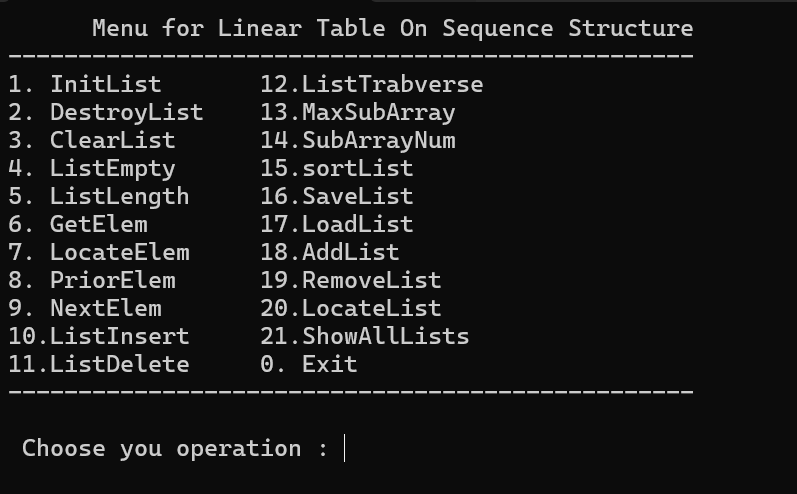
\includegraphics[width=0.8\textwidth]{images/菜单.png}
 	\caption{菜单}
 	\label{txlab}
 \end{figure}

测试集如下:

测试集1:线性表中存有元素1 2 3

测试集2:线性表集合中有两个线性表 表一: 1 3 5 ;表二: 2 4 6 

\setcounter{paragraph}{0}

\subsubsection{基本功能函数测试}

\paragraph{ 1.}InitList测试

测试1:测试函数是否能成功创建线性表;

测试2:测试当线性表已经存在时,函数是否能再次创建线性表。

\vspace{0.5em}

\begin{tabular}{|c|l|c|c|c|}
	\hline
	测试编号 & 测试输入 & 预期结果 & 实际运行结果 \\
	\hline
	1 & 1 & 线性表创建成功 & 一致 \\
	\hline
	2 & 1$\rightarrow$1 & 线性表创建失败 & 一致 \\
	\hline
\end{tabular}

~\

 \begin{figure}[H]
 	\centering
 	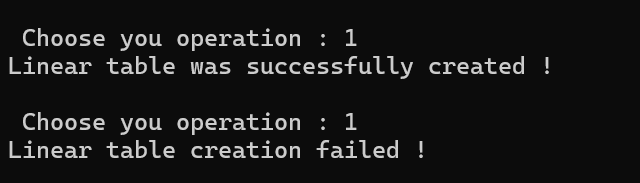
\includegraphics[width=0.6\textwidth]{images/线性表测试1.png}
 	\caption{测试1运行结果}
 	\label{txlab}
 \end{figure}


\paragraph{ 2.}DestroyList测试

测试1:测试函数是否能对不存在的线性表进行销毁;

测试2:测试函数是否能对已经存在的线性表进行销毁;

测试3:将测试在销毁线性表之后检测能否重新创建线性表。

\vspace{0.5em}

\begin{tabular}{|c|l|c|c|c|}
	\hline
	测试编号 & 测试输入 & 预期结果 & 实际运行结果 \\
	\hline
	1 & 2 & 线性表不存在,销毁失败 & 一致 \\
	\hline
	2 & 1$\rightarrow$2 & 线性表销毁成功 & 一致 \\
	\hline
	3 & 1$\rightarrow$2$\rightarrow$1 & 线性表销毁成功;线性表创建成功 & 一致 \\
	\hline
\end{tabular}

~\

 \begin{figure}[H]
 	\centering
 	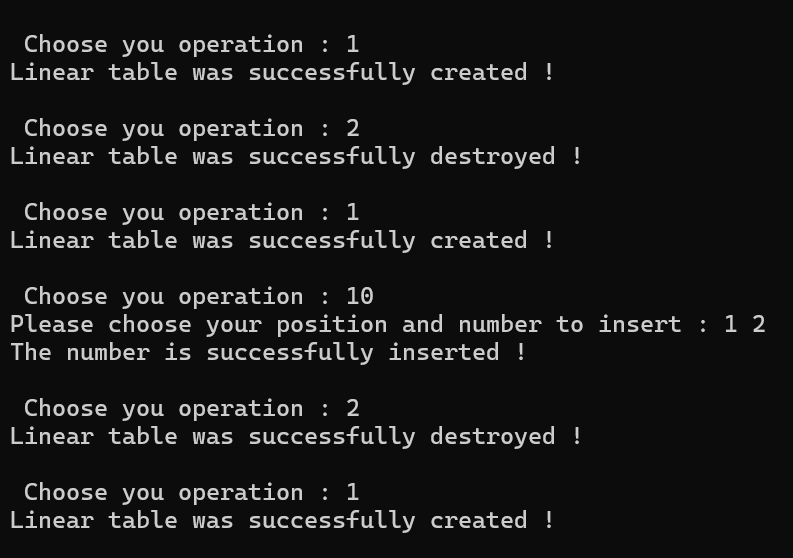
\includegraphics[width=0.6\textwidth]{images/线性表测试2.png}
 	\caption{测试2运行结果}
 	\label{txlab}
 \end{figure}


\paragraph{ 3.}ClearList测试

测试1:测试函数是否能对不存在的线性表进行清空;

测试2:测试函数是否能对已经存在的线性表进行清空;

测试3:在测试集1的情况下进行,在调用ClearList之后,通过求线性表的表长,来判断线性表中的元素是否确实被清空。

\vspace{0.5em}

\begin{tabular}{|c|l|c|c|c|}
	\hline
	测试编号 & 测试输入 & 预期结果 & 实际运行结果 \\
	\hline
	1 & 3 & 线性表不存在,清空失败 & 一致 \\
	\hline
	2 & 1$\rightarrow$3 & 线性表清空成功 & 一致 \\
	\hline
	3 & 1$\rightarrow$测试集1$\rightarrow$3$\rightarrow$5 & 线性表长度为0 & 一致 \\
	\hline
\end{tabular}

~\

 \begin{figure}[H]
 	\centering
 	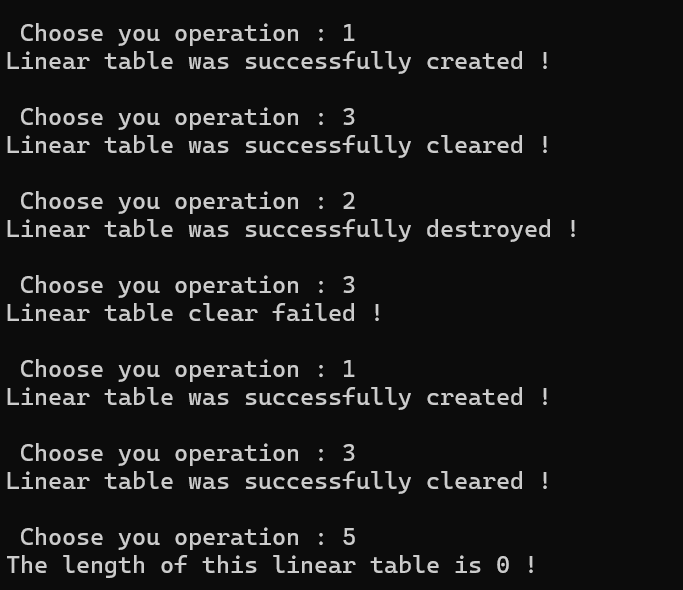
\includegraphics[width=0.6\textwidth]{images/线性表测试3.png}
 	\caption{测试3运行结果}
 	\label{txlab}
 \end{figure}


\paragraph{ 4.}ListEmpty测试

测试1:测试函数能否对不存在的线性表判空;

测试2:测试函数能否正确判断空线性表;

测试3:在测试集1的情况下进行,测试函数能否正确判断空线性表。

\vspace{0.5em}

\begin{tabular}{|c|l|c|c|c|}
	\hline
	测试编号 & 测试输入 & 预期结果 & 实际运行结果 \\
	\hline
	1 & 4 & 线性表不存在,判空失败 & 一致 \\
	\hline
	2 & 1$\rightarrow$4 & 线性表为空 & 一致 \\
	\hline
	3 & 1$\rightarrow$测试集1$\rightarrow$4 & 线性表非空 & 一致 \\
	\hline
\end{tabular}

~\

 \begin{figure}[H]
 	\centering
 	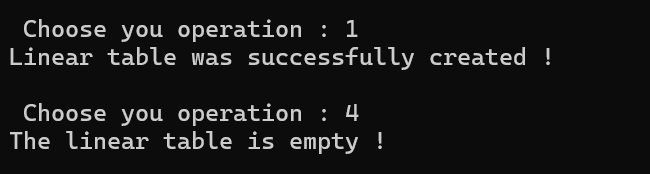
\includegraphics[width=0.6\textwidth]{images/线性表测试4.png}
 	\caption{测试4运行结果}
 	\label{txlab}
 \end{figure}


\paragraph{ 5.}ListLength测试


测试1:测试函数能否对不存在的线性表求长;

测试2:测试函数能否正确求出空线性表的长度;

测试3:在测试集1的情况下进行,测试函数能否正确求出线性表的长度。

\vspace{0.5em}

\begin{tabular}{|c|l|c|c|c|}
	\hline
	测试编号 & 测试输入 & 预期结果 & 实际运行结果 \\
	\hline
	1 & 5 & 线性表不存在,求长失败 & 一致 \\
	\hline
	2 & 1$\rightarrow$5 & 线性表长度为0 & 一致 \\
	\hline
	3 & 1$\rightarrow$测试集1$\rightarrow$5 & 线性表长度为3 & 一致 \\
	\hline
\end{tabular}

~\

 \begin{figure}[H]
 	\centering
 	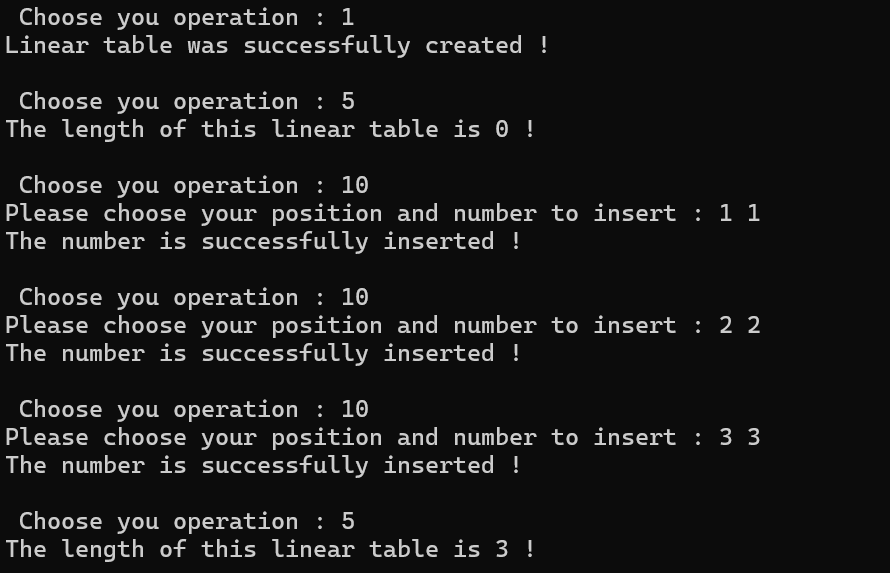
\includegraphics[width=0.6\textwidth]{images/线性表测试5.png}
 	\caption{测试1运行结果}
 	\label{txlab}
 \end{figure}


\paragraph{ 6.}GetElem测试

此函数的所有测试将在测试集1的情况下进行。

测试1,2:将测试函数能否正确找到元素;

测试3,4:将测试函数能否正确识别非法的位序。

\vspace{0.5em}

\begin{tabular}{|c|l|c|c|}
	\hline
	测试编号 & 测试输入 & 预期结果 & 实际运行结果 \\
	\hline
	1 & 6$\rightarrow$2 & 线性表中第2个元素为2 & 一致 \\
	\hline
	2 & 6$\rightarrow$5 & 线性表中第3个元素为3 & 一致 \\
	\hline
	3 & 6$\rightarrow$-1 & 输入的逻辑索引不合法! & 一致 \\
	\hline
	4 & 6$\rightarrow$5 & 输入的逻辑索引不合法! & 一致 \\
	\hline
\end{tabular}

~\

 \begin{figure}[H]
 	\centering
 	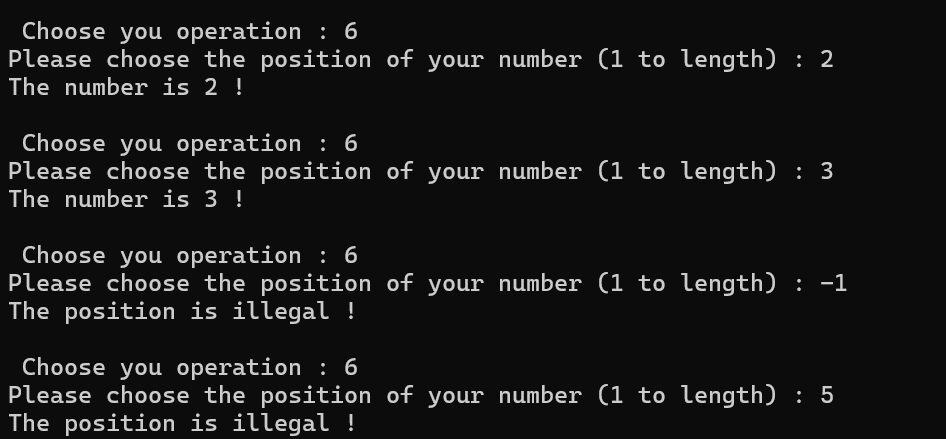
\includegraphics[width=0.6\textwidth]{images/线性表测试6.png}
 	\caption{测试2运行结果}
 	\label{txlab}
 \end{figure}

\paragraph{ 7.}LocateElem测试

此函数的所有测试将在测试集1的情况下进行。

测试1:将测试函数能否正确找到位序;

测试3,4:将测试函数能否正确识别不在线性表中的元素。

\vspace{0.5em}

\begin{tabular}{|c|l|c|c|}
	\hline
	测试编号 & 测试输入 & 预期结果 & 实际运行结果 \\
	\hline
	1 & 7$\rightarrow$1 & 该元素存在且元素逻辑索引为:1 & 一致 \\
	\hline
	3 & 7$\rightarrow$5 & 输入的元素不存在! & 一致 \\
	\hline
	4 & 7$\rightarrow$-1 & 输入的元素不存在! & 一致 \\
	\hline
\end{tabular}

~\

 \begin{figure}[H]
 	\centering
 	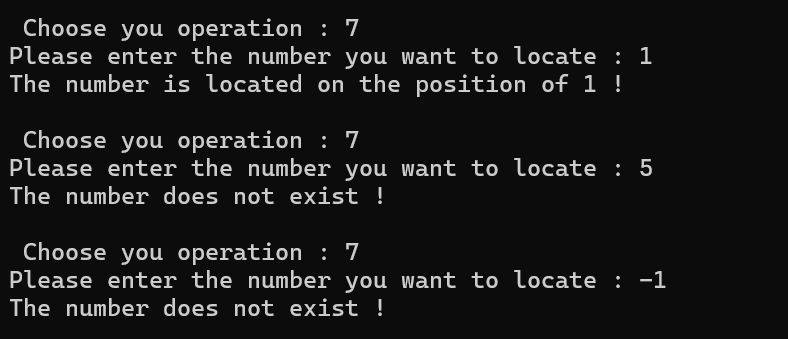
\includegraphics[width=0.6\textwidth]{images/线性表测试7.png}
 	\caption{测试2运行结果}
 	\label{txlab}
 \end{figure}


\paragraph{ 8.}PriorElem测试

    此函数的所有测试将在测试集1的情况下进行。

    测试1:将测试函数能否正确找到前驱;

    测试2:将测试函数能否正确判断第一个元素没有前驱;

    测试3:将测试函数能否正确判断不在线性表中的元素没有前驱。

\vspace{0.5em}

\begin{tabular}{|c|l|c|c|}
	\hline
	测试编号 & 测试输入 & 预期结果 & 实际运行结果 \\
	\hline
	1 & 8$\rightarrow$2 & 该元素存在且前驱元素为:1 & 一致 \\
	\hline
	2 & 8$\rightarrow$1 & 线性表中该元素不存在前驱! & 一致 \\
	\hline
	3 & 8$\rightarrow$4 & 线性表中该元素不存在! & 一致 \\
	\hline
\end{tabular}

~\

 \begin{figure}[H]
 	\centering
 	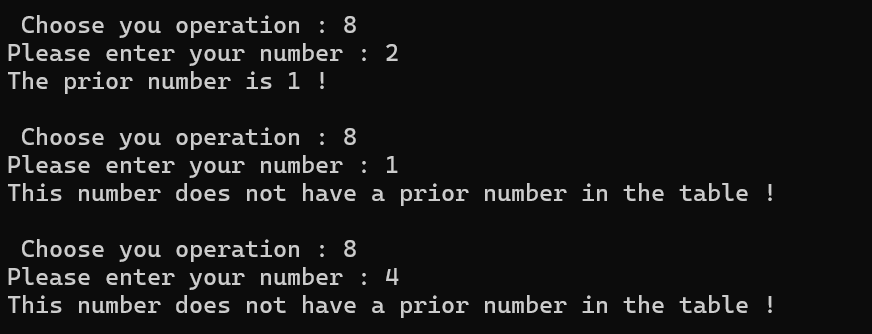
\includegraphics[width=0.6\textwidth]{images/线性表测试8.png}
 	\caption{测试2运行结果}
 	\label{txlab}
 \end{figure}


\paragraph{ 9.}NextElem测试

    此函数的所有测试将在测试集1的情况下进行。

    测试1:将测试函数能否正确找到后继;

    测试2:将测试函数能否正确判断最后一个元素没有后继;

    测试3:将测试函数能否正确判断不在线性表中的元素没有后继。

\vspace{0.5em}

\begin{tabular}{|c|l|c|c|}
	\hline
	测试编号 & 测试输入 & 预期结果 & 实际运行结果 \\
	\hline
	1 & 9$\rightarrow$2 & 线性表中该元素的后继为3 & 一致 \\
	\hline
	2 & 9$\rightarrow$3 & 线性表中该元素不存在后继! & 一致 \\
	\hline
	3 & 9$\rightarrow$4 & 线性表中该元素不存在! & 一致 \\
	\hline
\end{tabular}

~\

 \begin{figure}[H]
 	\centering
 	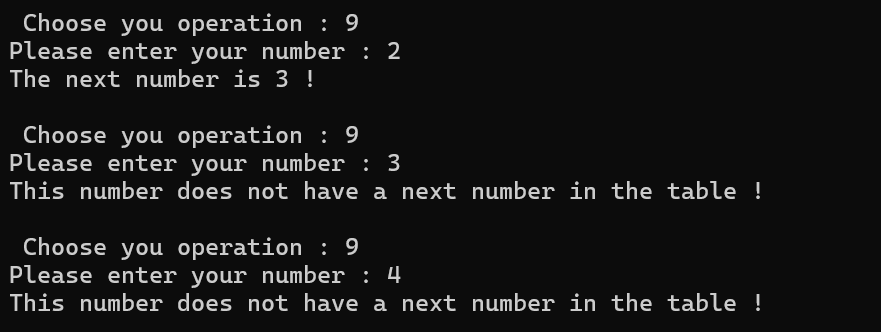
\includegraphics[width=0.6\textwidth]{images/线性表测试9.png}
 	\caption{测试2运行结果}
 	\label{txlab}
 \end{figure}


\paragraph{10.}ListInsert测试

	输入要求:依次输入插入元素位置和插入元素。

	测试1在空线性表的情况下进行,通过反复调用函数来构建测试集1(1 2 3),将通过遍历线性表和求表长来检验插入是否正确;

	测试2,3将在测试1的基础上进行,测试函数能否正确判断线性表两端非法的插入位置;

\vspace{0.5em}

\begin{tabular}{|c|p{2.8cm}|p{5cm}|c|}
	\hline
	测试编号 & 测试输入 & 预期结果 & 实际运行结果 \\
	\hline
	1 & 10$\rightarrow$1 1$\rightarrow$10$\rightarrow$2 2$\rightarrow$10$\rightarrow$3 3 & 线性表插入成功! & 一致 \\
	\hline
	2 & 10$\rightarrow$7 & 插入位置不合法,线性表插入失败! & 一致 \\
	\hline
	3 & 10$\rightarrow$0 & 插入位置不合法,线性表插入失败! & 一致 \\
	\hline
\end{tabular}

~\

 \begin{figure}[H]
 	\centering
 	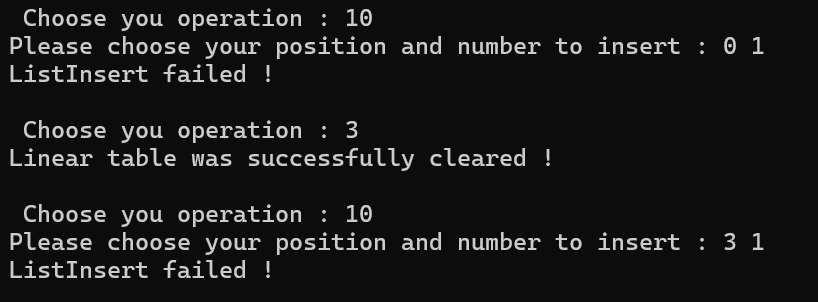
\includegraphics[width=0.6\textwidth]{images/线性表测试10.png}
 	\caption{测试2运行结果}
 	\label{txlab}
 \end{figure}


\paragraph{11.}ListDelete测试

	输入要求:输入删除的序号

	此函数的所有测试将在测试集1的情况下进行,进行一项测试后,不恢复至测试集1的状态。

	测试1:将测试函数能否正确判断非法的序号;

	测试2:将测试函数能否正确删除元素,采用遍历的方式检验正确性;


\vspace{0.5em}

\begin{tabular}{|c|p{2.7cm}|p{4.5cm}|c|}
	\hline
	测试编号 & 测试输入 & 预期结果 & 实际运行结果 \\
	\hline
	1 & 11$\rightarrow$0 & 删除位置不合法! & 一致 \\
	\hline
	2 & 11$\rightarrow$2$\rightarrow$2 & 元素已删除!遍历后的结果为1 3 & 一致 \\
	\hline
\end{tabular}

~\

 \begin{figure}[H]
 	\centering
 	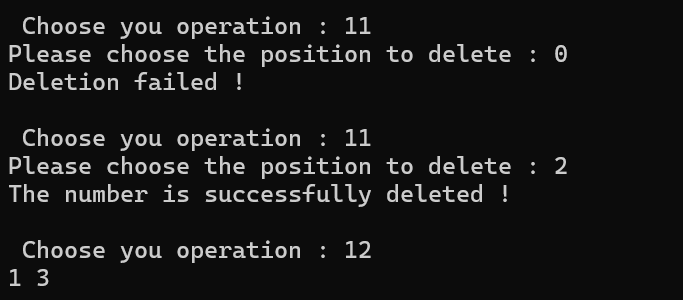
\includegraphics[width=0.6\textwidth]{images/线性表测试11.png}
 	\caption{测试2运行结果}
 	\label{txlab}
 \end{figure}


\paragraph{12.}ListTraverse测试

	测试1在线性表是空表的情况下进行,测试函数能否处理空表的情况;

	测试2在测试集1的情况下进行,测试函数能否正确遍历线性表。

\vspace{0.5em}

\begin{tabular}{|c|p{2.7cm}|c|c|}
	\hline
	测试编号 & 测试输入 & 预期结果 & 实际运行结果 \\
	\hline
	1 & 3$\rightarrow$12 & 线性表是空表 & 一致 \\
	\hline
	2 & 12 & 1 2 3 & 一致 \\
	\hline
\end{tabular}

~\

 \begin{figure}[H]
 	\centering
 	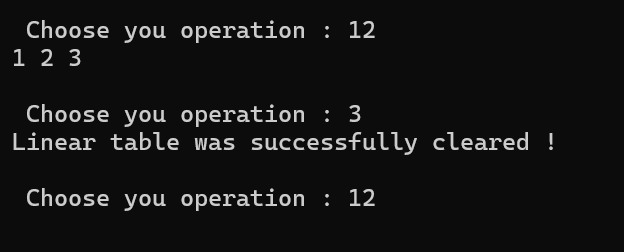
\includegraphics[width=0.6\textwidth]{images/线性表测试12.png}
 	\caption{测试2运行结果}
 	\label{txlab}
 \end{figure}


\subsubsection{附加功能测试}

\paragraph{13.}MaxSubArray测试

测试1:在没有创建线性表的情况下进行,测试函数能否正确判断线性表的存在性;
	
测试2:在测试集1的情况下进行,测试函数能否实现求最大连续子数组和的功能。

\vspace{0.5em}

\begin{tabular}{|c|p{2.7cm}|c|c|}
	\hline
	测试编号 & 测试输入 & 预期结果 & 实际运行结果 \\
	\hline
	1 & 2$\rightarrow$13 & 线性表未创建! & 一致 \\
	\hline
	2 & 13 & 最大子数组之和为: 6& 一致 \\
	\hline
\end{tabular}

~\

 \begin{figure}[H]
 	\centering
 	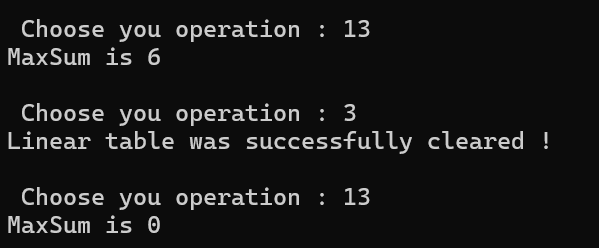
\includegraphics[width=0.6\textwidth]{images/线性表测试13.png}
 	\caption{测试2运行结果}
 	\label{txlab}
 \end{figure}


\paragraph{14.}SubArrayNum测试
	
测试1:在没有创建线性表的情况下进行,测试函数能否正确判断线性表的存在性;

测试2:在测试集1的情况下进行,测试函数能否实现计数和为K的子数组的功能。

\vspace{0.5em}

\begin{tabular}{|c|p{2.7cm}|c|c|}
	\hline
	测试编号 & 测试输入 & 预期结果 & 实际运行结果 \\
	\hline
	1 & 2$\rightarrow$14 & 线性表未创建! & 一致 \\
	\hline
	2 & 14$\rightarrow$3 & 和为数3的连续数组数目为:2 & 一致 \\
	\hline
\end{tabular}

~\

 \begin{figure}[H]
 	\centering
 	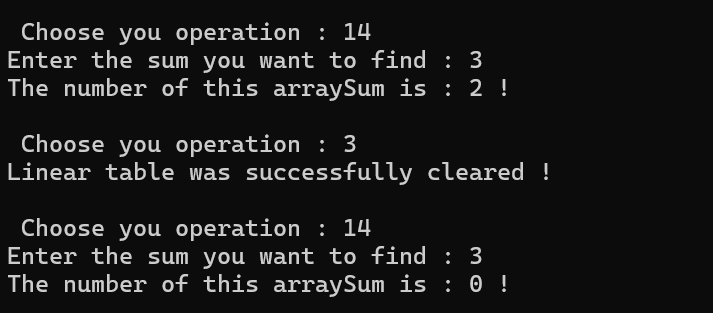
\includegraphics[width=0.6\textwidth]{images/线性表测试14.png}
 	\caption{测试2运行结果}
 	\label{txlab}
 \end{figure}

\paragraph{15.}sortList测试

测试1:在线性表存在的情况下进行,测试函数能否正确排序。

\vspace{0.5em}

\begin{tabular}{|c|p{2.7cm}|c|c|}
	\hline
	测试编号 & 测试输入 & 预期结果 & 实际运行结果 \\
	\hline
	1 & 12$\rightarrow$15$\rightarrow$12 & 1 2 3 & 一致 \\
	\hline
\end{tabular}

~\

 \begin{figure}[H]
 	\centering
 	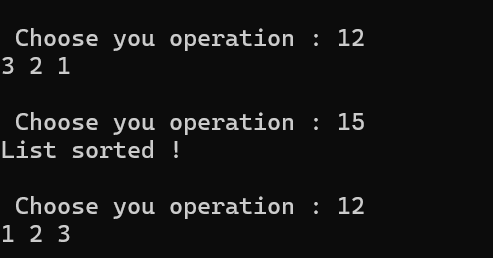
\includegraphics[width=0.6\textwidth]{images/线性表测试15.png}
 	\caption{测试2运行结果}
 	\label{txlab}
 \end{figure}


\paragraph{16.}SaveList测试
	
测试1:在测试集1的情况下进行,测试函数能否正常进行写文件操作;

\vspace{0.5em}

\begin{tabular}{|c|p{2.7cm}|c|c|}
	\hline
	测试编号 & 测试输入 & 预期结果 & 实际运行结果 \\
	\hline
	1 & 16$\rightarrow$list1.txt & 文件保存成功! & 一致 \\
	\hline
\end{tabular}

~\

\paragraph{17.}LoadList测试
	
本函数的测试都在文件1中已存有测试集1的情况下进行。

测试1:在线性表不存在的情况下进行,测试函数能否正确进行读文件操作,采用遍历线性表的方式检验正确性。

\vspace{0.5em}

\begin{tabular}{|c|p{2.7cm}|c|c|}
	\hline
	测试编号 & 测试输入 & 预期结果 & 实际运行结果 \\
	\hline
	1 & 17$\rightarrow$list1.txt & 文件录入成功!遍历:1 2 3 & 一致 \\
	\hline
\end{tabular}

~\

\paragraph{18.}AddList测试

测试1:构建测试集2,测试线性表能否正确添加,通过遍历各个表检验正确性。

\vspace{0.5em}

\begin{tabular}{|c|p{2.7cm}|c|c|}
	\hline
	测试编号 & 测试输入 & 预期结果 & 实际运行结果 \\
	\hline
	1 & 18 & 表一 表二 & 一致 \\
	\hline
\end{tabular}

~\

 \begin{figure}[H]
 	\centering
 	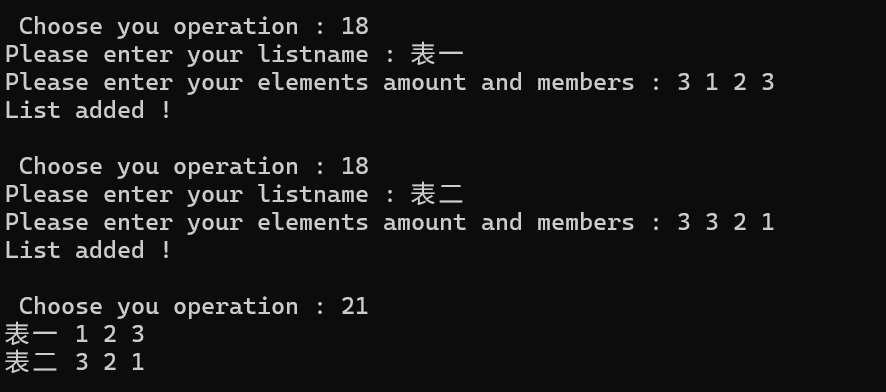
\includegraphics[width=0.6\textwidth]{images/线性表测试18.png}
 	\caption{测试2运行结果}
 	\label{txlab}
 \end{figure}

\paragraph{19.}RemoveList测试

本函数的测试在测试集2的基础上进行。

测试1:将测试函数能否正确删除线性表,采用遍历各线性表的方式判断正确性;

测试2:在测试1的基础上进行,尝试删除一个不在集合中的线性表,测试函数能否给出正确判断。

\vspace{0.5em}

\begin{tabular}{|c|p{2.7cm}|c|c|}
	\hline
	测试编号 & 测试输入 & 预期结果 & 实际运行结果 \\
	\hline
	1 & 19$\rightarrow$表一 & 表一已成功删除! & 一致 \\
	\hline
	2 & 19$\rightarrow$表三 & 线性表不存在! & 一致 \\
	\hline
\end{tabular}

~\

 \begin{figure}[H]
 	\centering
 	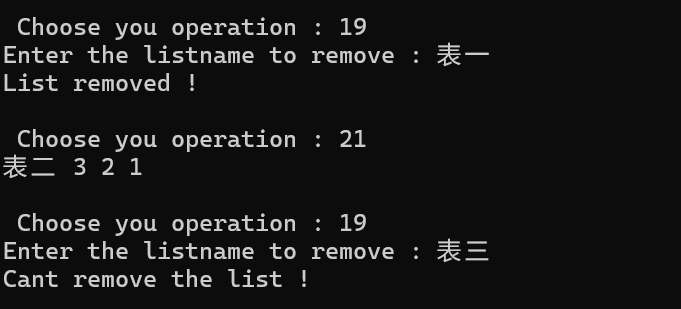
\includegraphics[width=0.6\textwidth]{images/线性表测试19.png}
 	\caption{测试2运行结果}
 	\label{txlab}
 \end{figure}

\paragraph{20.}LocateList测试
	
本函数的测试在测试集2的基础上进行。

测试1:将测试函数能否正确定位线性表;

测试2:将尝试查找一个不在集合中的线性表,测试函数能否给出正确判断。

\vspace{0.5em}

\begin{tabular}{|c|p{2.7cm}|c|c|}
	\hline
	测试编号 & 测试输入 & 预期结果 & 实际运行结果 \\
	\hline
	1 & 20$\rightarrow$表一 & 该线性表的逻辑索引为:1 & 一致 \\
	\hline
	2 & 20$\rightarrow$表三 & 线性表查找失败! & 一致 \\
	\hline
\end{tabular}

~\

 \begin{figure}[H]
 	\centering
 	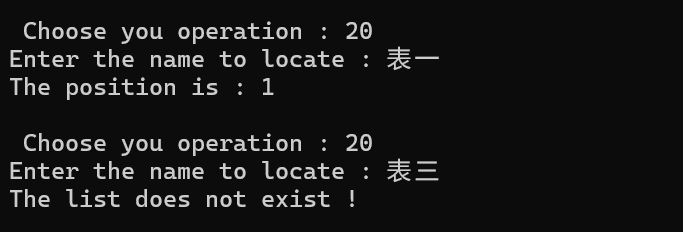
\includegraphics[width=0.6\textwidth]{images/线性表测试20.png}
 	\caption{测试2运行结果}
 	\label{txlab}
 \end{figure}


\paragraph{21.}TraverseList测试
	
测试1:在测试集2的基础上进行,测试函数能否正确遍历各个线性表;

\vspace{0.5em}

\begin{tabular}{|c|p{2.7cm}|c|c|}
	\hline
	测试编号 & 测试输入 & 预期结果 & 实际运行结果 \\
	\hline
	1 & (测试集3)21 & 表一 表二 & 一致 \\
	\hline
\end{tabular}

~\

测试小结

21个函数基本符合了测试要求,在正常和异常用例的条件下均可以正常运行。

\subsection{实验小结}

本次实验让我加深了对线性表的概念、基本运算的理解,掌握了线性表的基本运算的实现,熟练了线性表的逻辑结构和物理结构的关系。

在编写程序和测试的过程中,遇到了诸多问题,例如如何设计多线性表操作,如何保证能够单独对某一线性表进行基本操作。解决方案是将其完整赋值给主函数中的
全局变量,保证了集合中表的独立性,可以不受主函数中操作的影响,表之间可以分立进行。

在今后的学习过程当中应该更多地从数据结构的角度去分析如何进行数据的存储、读取和处理,如何设计便于存储的数据结构,同时应具有开放性思维,设计高性能的算法,以达到更简便地解决实际问题的目的。同时,以后还需要多加练习,以达到熟能生巧的效果。

\newpage

\section{基于二叉链表的二叉树实现}

\subsection{问题描述}

采用二叉链表作为二叉树的物理结构,实现基本运算。ElemType为数据元素的类型名,具体含义可自行定义,但要求二叉树结点类型为结构型,至少包含二个部分,一个是能唯一标识一个结点的关键字(类似于学号或职工号),另一个是其它部分。

要求构造一个具有菜单的功能演示系统。其中,在主程序中完成函数调用所需实参值的准备和函数执行结果的显示,并给出适当的操作提示显示。

演示系统可选择实现二叉树的文件形式保存。其中,\whiteding{1}需要设计文件数据记录格式,以高效保存二叉树数据逻辑结构(D,{R})的完整信息;\whiteding{2}需要设计二叉树文件保存和加载操作合理模式。附录B提供了文件存取的方法。
演示系统可选择实现多个二叉树管理。可采用线性表的方式管理多个二叉树,线性表中的每个数据元素为一个二叉树的基本属性,至少应包含有二叉树的名称。

演示系统的源程序应按照代码规范增加注释和排版,目标程序务必是可以独立于IDE运行的EXE文件。

\subsection{系统设计}

\subsubsection{头文件和预定义}

1、头文件

\begin{lstlisting}[language=c]
#include "stdio.h"
#include "stdlib.h"
#include <malloc.h>
#include <string.h>
\end{lstlisting}

2、预定义常量

\begin{lstlisting}[language=c]
#define TRUE 1
#define FALSE 0
#define OK 1
#define ERROR 0
#define INFEASIBLE -1
#define OVERFLOW -2
#define MAXlength 10

\end{lstlisting}

3、类型表达式

\begin{lstlisting}[language=c]
typedef int status;
typedef int KeyType;
typedef struct {
    KeyType key;
    char others[20];
} TElemType; // 二叉树结点类型定义
typedef struct BiTNode { // 二叉链表结点的定义
    TElemType data;
    struct BiTNode *lchild, *rchild;
} BiTNode, *BiTree;
typedef struct {
    struct {
        char name[20];
        BiTree T;
    } elem[10];
    int amount;
} Trees;
typedef struct {
    int pos;
    TElemType data;
} DEF;
\end{lstlisting}

\subsubsection{基本功能函数}

 \begin{figure}[H]
 	\centering
 	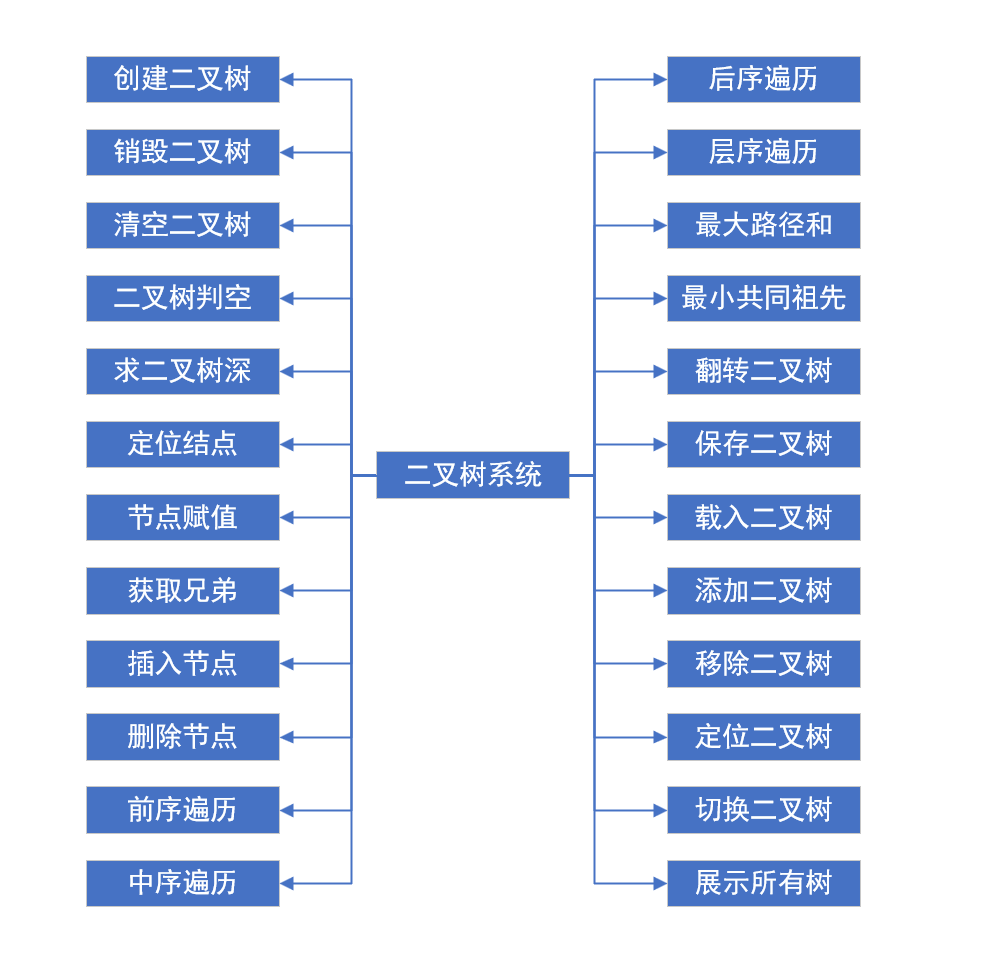
\includegraphics[width=0.9\textwidth]{images/二叉树系统.png}
 	\caption{系统整体功能设计图}
 	\label{txlab}
 \end{figure}

\begin{enumerate}
    \item 创建二叉树:函数名称是CreateBiTree(T,definition);初始条件是definition 给出二叉树T的定义;操作结果是按definition构造二叉树T;
    \item 销毁二叉树:函数名称是DestroyBiTree(T);初始条件是二叉树T已存在;操作结果是销毁二叉树T;
    \item 清空二叉树:函数名称是ClearBiTree (T);初始条件是二叉树T存在;操作结果是将二叉树T清空;
    \item 判定空二叉树:函数名称是BiTreeEmpty(T);初始条件是二叉树T存在;操作结果是若T为空二叉树则返回TRUE,否则返回FALSE;
    \item 求二叉树深度:函数名称是BiTreeDepth(T);初始条件是二叉树T存在;操作结果是返回T的深度;
    \item 查找结点:函数名称是LocateNode(T,e);初始条件是二叉树T存在,e是和T中结点关键字类型相同的值;操作结果是返回查找到的结点指针,否则返回NULL;
    \item 结点赋值:函数名称是Assign(T,e,value);初始条件是二叉树T已存在,e是和T中结点关键字类型相同的值;操作结果是关键字为e的结点赋值为value,返回OK,否则返回FALSE;
	\item 获得兄弟结点:函数名称是GetSibling(T,e);初始条件是二叉树T存在,e是和T中结点关键字类型相同的值;操作结果是返回关键字为e的结点的兄弟结点指针。否则返回NULL;
	\item 插入结点:函数名称是InsertNode(T,e,LR,c);初始条件是二叉树T存在,e是和T中结点关键字类型相同的值,LR为0或1,c是待插入结点;操作结果是根据LR为0或者1,插入结点c到T中,作为关键字为e的结点的左或右孩子结点,结点e的原有左子树或右子树则为结点c的右子树;当LR为-1时新增节点作为根节点,原树作为该节点的右子树,操作成功返回OK,否则返回FALSE。
	\item 删除结点:函数名称是DeleteNode(T,e);初始条件是二叉树T存在,e是和T中结点关键字类型相同的值。操作结果是删除T中关键字为e的结点;同时,如果关键字为e的结点度为0,删除即可;如关键字为e的结点度为1,用关键字为e的结点孩子代替被删除的e位置;如关键字为e的结点度为2,用e的左孩子代替被删除的e位置,e的右子树作为e的左子树中最右结点的右子树;
	\item 前序遍历:函数名称是PreOrderTraverse(T,Visit());(本系统前序遍历采用非递归算法)初始条件是二叉树T存在,Visit是一个函数指针的形参;操作结果是先序遍历,对每个结点调用函数Visit一次且一次,一旦调用失败,则操作失败。
	\item 中序遍历:函数名称是InOrderTraverse(T,Visit());初始条件是二叉树T存在,Visit是一个函数指针的形参;操作结果是中序遍历,对每个结点调用函数Visit一次且一次,一旦调用失败,则操作失败;
	\item 后序遍历:函数名称是PostOrderTraverse(T,Visit());初始条件是二叉树T存在,Visit是一个函数指针的形参;操作结果是后序遍历,对每个结点调用函数Visit一次且一次,一旦调用失败,则操作失败。
	\item 按层遍历:函数名称是LevelOrderTraverse(T,Visit());初始条件是二叉树T存在,Visit是一个函数指针的形参;操作结果是层序遍历,对每个结点调用函数Visit一次且一次,一旦调用失败,则操作失败。
\end{enumerate}

\subsubsection{附加功能函数}

\begin{enumerate}
    \item 最大路径和:函数名称是MaxPathSum(T),初始条件是二叉树T存在;操作结果是返回根节点到叶子结点的最大路径和;
    \item 最近公共祖先:函数名称是LowestCommonAncestor(T,e1,e2);初始条件是二叉树T存在;操作结果是该二叉树中e1节点和e2节点的最近公共祖先;
    \item 翻转二叉树:函数名称是InvertTree(T),初始条件是线性表L已存在;操作结果是将T翻转,使其所有节点的左右节点互换;
	\item 文件写入:函数名称是 SaveBiTree(T,FileName);初始条件是二叉树T已存在;操作结果是将T的元素写到名称为FileName的文件中。
	\item 文件读出:函数名称是 LoadBiTree(T,FileName);初始条件是二叉树T不存在;操作结果是将文件FileName中的内容载入到新表 T中。
    \item 实现多个二叉树管理:设计相应的数据结构管理多个二叉树的查找、添加、移除、切换、展示功能。
	\begin{enumerate}
	\item 增加二叉树:函数名称是AddBiTree(trees, TreeName);初始条件是名称为TreeName的二叉树不存在于二叉树集合中;操作结果是在trees中创建一个名称为TreeName的二叉树。
	\item 移除二叉树:函数名称是RemoveBiTree(trees, TreeName);初始条件是名称为TreeName的二叉树存在于二叉树集合中;操作结果是将该二叉树移除。
	\item 查找二叉树:函数名称是LocateBiTree(trees, TreeName);初始条件是名称为TreeName的二叉树存在于二叉树集合中;操作结果是返回该二叉树在trees中的逻辑索引。
	\item 切换二叉树:函数名称是SwitchTrees(trees,TreeName,T);初始条件是名称为TreeName的二叉树已存在于二叉树集合中;操作结果是将该树调转为当前操作的树T。
	\item 遍历所有表:函数名称是ShowAllTrees(trees);初始条件是trees已存在;操作结果是对所有的二叉树依次进行前序和中序遍历。
	\end{enumerate}
\end{enumerate}

\subsubsection{演示系统}

构造一个具有菜单的功能演示系统。其中,在主程序中完成函数调用所需实参值的准备和函数执行结果的显示,并给出适当的操作提示显示。演示系统可选择实现二叉树的文件形式保存。其中,\whiteding{1}需要设计文件数据记录格式,以高效保存二叉树数据逻辑结构(D,[R])的完整信息;\whiteding{2}需要设计二叉树文件保存和加载操作合理模式。演示系统实现了多个二叉树管理。
    输入1$\sim$24可以调用上述的24个函数,对二叉树或二叉树集合进行操作;输入0时退出系统。

该演示系统具有完备性,包含每一功能的中英文说明和注意事项,同时显示当前二叉树名称和初始化情况。

下面是该系统的初始界面

 \begin{figure}[H]
 	\centering
 	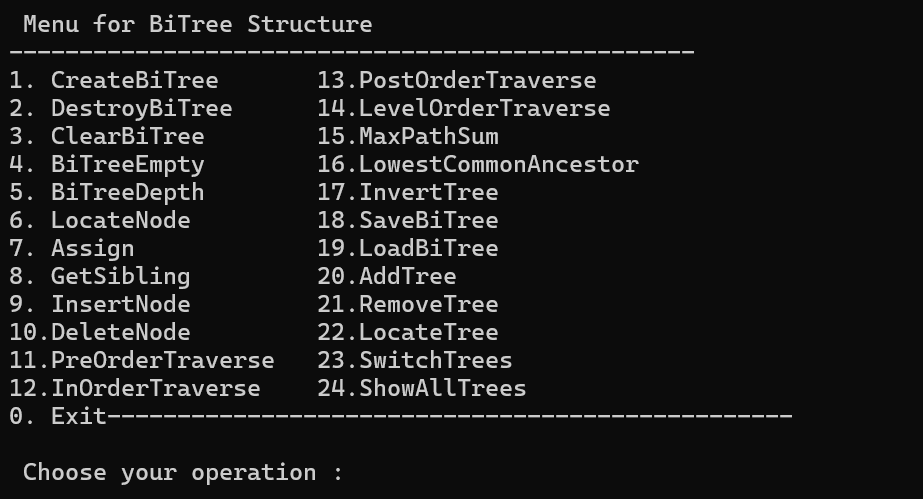
\includegraphics[width=0.9\textwidth]{images/二叉树系统界面.png}
 	\caption{系统整体界面}
 	\label{txlab}
 \end{figure}


\subsection{系统实现}

\subsubsection{演示系统框架}

系统主体通过while循环实现多次选择,通过op获取用户的选择,通过switch语句根据用户选择实现具体功能。

具体实现为将菜单和功能实现写入到 while 循环中,用op 获取用户的选择,op初始化为 1,以便第一次能进入循环。进入循环后,用户输入选择 0$\sim$24,其中 1$\sim$24 分别代表二叉树的一个基本操作,在主函数中通过 switch语句对应到相应的函数功能,执行完该功能后通过 break 跳出switch 语句,继续执行 while 循环,直至用户输入 0 退出当前演示系统。

\subsubsection{函数思想及实现}

\setcounter{paragraph}{0}

二叉树基本功能函数的实现:

\paragraph{ 1.} status CreateBiTree(BiTree \&T, TElemType definition[])

输入:二叉树T,TELemType类型数组

输出:创建二叉树的状态

函数思想描述:创建二叉树函数,传入二叉树和TELemType类型数组。根据defination的位置判断奇偶来确定左右子树,最后将T赋值根节点,从而构建二叉树。

\paragraph{ 2.} status DestroyBiTree(BiTree \&T)
    
输入:二叉树T

输出:二叉树销毁状态

函数思想描述:销毁二叉树函数,将二叉树设置成空,并删除所有结点,释放结点空间。在函数中,如果当前结点有左子树或右子树,则递归调用本函数依次销毁当前结点的左子树和右子树;如果当前结点的左右子树都为空指针时释放当前结点的存储空间,并将当前结点的指针设置为 NULL。

\paragraph{ 3.}status ClearBiTree(BiTree \&T)
    
输入:二叉树T

输出:二叉树清空状态

函数思想描述:清空二叉树函数,将二叉树设置成空。在函数中,如果当前结点有左子树或右子树,则递归调用本函数依次清空当前结点的左子树和右子树。

\paragraph{ 4.}status BiTreeEmpty(BiTree T)

输入:二叉树T

输出:二叉树是否为空

函数思想描述:判断树是否为空,如果根结点为空,则返回TRUE,否则说明树非空,返回FALSE。

\paragraph{ 5.}int BiTreeDepth(BiTree T)

输入:二叉树T

输出:二叉树的深度

函数思想概述:求二叉树深度函数,依次遍历二叉树的左右结点,遇到空结点则返回0,不断比较获取二叉树到叶子结点的深度的较大值,作为二叉树的深度,最终结果即为二叉树深度。

\paragraph{ 6.}BiTNode *LocateNode(BiTree T, KeyType e)

输入:二叉树T,KeyType e

输出:二叉树结点指针

函数思想描述:查找二叉树中关键字结点函数,使用递归思想,若当前结点为目标结点,则返回当前结点的地址值;若当前结点指针为空,则说明此子树都没有所找结点,返回 NULL 指针;否则依次递归查找左右子树中是否有目标结点,并记录在左右子树查找的返回值。整个函数的返回值若为NULL,则说明整棵树没有目标结点,否则返回目标结点。

\paragraph{ 7.}status Assign(BiTree \&T, KeyType e, TElemType value)

输入:二叉树T,KeyType e,TElemType value

输出:赋值状态

函数思想描述:结点赋值函数,首先通过LocateNode函数查找用以替换的结点的关键字与除被替换结点以外的其他结点的关键字是否有重复,若重复则返回 ERROR。若无重复则调用 LocateNode 函数查找被替换结点,若未找到则返回 ERROR;若找到,则对该结点的关键字和关键信息进行赋值,并返回OK。

\paragraph{ 8.}BiTNode *GetSibling(BiTree T, KeyType e)

输入:二叉树T,KeyType e

输出:二叉树兄弟结点指针

函数思想概述:获得当前结点的兄弟结点函数,使用了递归思想,若当前结点为空则说明为空树,若当前结点无左右子树则说明当前结点不符合条件,返回 NULL;若当前结点有左右子树,则若左右子树其一结点关键字为所求,且另一子树存在,则找到兄弟结点,返回兄弟结点指针,若另一子树不存在,则该节点没有兄弟结点,返回 NULL;若当前结点的左右子树都不为指定节点,则递归调用此函数在左右子树中查找,并记录返回结果。整个函数若最终返回值为NULL 则说明该树没有此结点或此结点无兄弟节点;若返回值不为 NULL 则说明在某一子树中找到了指定节点的兄弟结点,返回该结点的值。

\paragraph{ 9.}status InsertNode(BiTree \&T, KeyType e, int LR, TElemType c)

输入:二叉树T,KeyType e,整型变量 LR ,TElemType c

输出:结点插入状态

函数思想概述:插入结点函数,首先通过LocateNode 函数判断待插入结点在树中有无关键字重复,若有则返回 ERROR,若无重复则调用 LocateNode 函数查找被插入结点,然后根据 LR 为 0 或者 1,插入结点 c 到 T 中,作为关键字为 e 的结点的左或右孩子结点,结点 e 的原有左子树或右子树则为结点 c 的右子树,返回 OK。如果插入失败,返回 ERROR。特别地,当 LR 为-1 时,作为根结点插入,原根结点作为 c 的右子树,最后返回 OK。

\paragraph{10.}status DeleteNode(BiTree \&T, KeyType e)

输入:二叉树T,KeyType e

输出:节点删除状态

函数思想概述:删除结点函数,e 是 T 中结点关键字类型相同的给定值。删除 T 中关键字为 e 的结点;如果关键字为 e 的结点度为 0,删除即可;如关键字为 e 的结点度为 1,用关键字为 e 的结点孩子代替被删除的 e 位置;如关键字为 e 的结点度为 2,用 e 的左孩子代替被删除的 e 位置,e 的右子树作为 e 的左子树中最右结点的右子树。成功删除结点后返回 OK,否则返回ERROR。

\paragraph{11.}status PreOrderTraverse(BiTree T, void (*visit)(BiTree))

输入:二叉树T,函数指针*visit

输出:前序遍历状态

函数思想概述:先序遍历函数,采用了非递归算法。在函数中,若当前结点为空,则返回 ERROR;若当前结点不为空,则首先通过visit访问当前结点,然后利用栈的特性依次对左右子树结点进栈出栈实现遍历。

\paragraph{12.}status InOrderTraverse(BiTree T, void (*visit)(BiTree))

输入:二叉树T,函数指针*visit

输出:中序遍历状态

函数思想概述:中序遍历函数,用递归算法实现。在函数中,若当前结点为空,则返回 ERROR;若当前结点不为空,则首先递归调用本函数依次中序遍历当前结点的左子树,根节点和右子树。

\paragraph{13.}status PostOrderTraverse(BiTree T, void (*visit)(BiTree))

输入:二叉树T,函数指针*visit

输出:后序遍历状态

函数思想概述:后序遍历函数,采用了递归思想。在函数中,若当前结点为空,则返回 ERROR;若当前结点不为空,则首先递归调用本函数依次后序遍历当前结点的左子树和右子树,然后访问当前结点。

\paragraph{14.}status LevelOrderTraverse(BiTree T, void (*visit)(BiTree))

输入:二叉树T,函数指针*visit

输出:层序遍历状态

函数思想概述:层序遍历函数,用非递归形式实现,调用队列数据结构和相应操作函数。在函数中,首先定义并初始化队列,然后定义 p 为根节点,并将根结点进队列。然后开始循环,该循环在队列为空时结束:首先将根节点出队列,若此节点不为空则访问该结点并依次将该结点的左右子树进队列,该循环结束则说明已经遍历完所有结点。在队列中,根节点下一层的子树先进队列。再依此顺序将左右子树的下一层子树再进队列,以此类推,直到最后一层子树。所以在每一层内的遍历顺序为从左向右。

附加功能函数的实现:

\paragraph{15.}int MaxPathSum(BiTree T)

输入:二叉树T

输出:最大路径和

函数思想描述:最大路径和函数,通过不断递归到叶子节点到空树,比较左右子节点的大小,选择较大值直到无法继续,然后返回路径上的最大值。

\paragraph{16.}BiTree LowestCommonAncestor(BiTree T, int e1, int e2)

输入:二叉树T,整型变量 e1,整型变量 e2

输出:二叉树结点:最近公共祖先

函数思想描述:递归查找左子树和右子树,若查找到目标结点,则返回该结点的指针,若查找到空树,则返回NULL。然后判断若左结点的返回值和右节点的返回值均不为NULL,则返回该结点,若左结点和右节点存在一个结点不为空,则返回该结点;否则返回NULL。最终返回的结点为两结点的最近公共祖先。

时间复杂度:O(nlogn)

空间复杂度:O(1)

\paragraph{17.}status InvertTree(BiTree \&T)

输入:二叉树T

输出:函数运行状态

函数思想描述:将二叉树翻转写成函数,以递归形式实现,依次交换左右子树直至无法交换,最终得到翻转后的二叉树。

时间复杂度:O(nlogn)

空间复杂度:O(1)

\paragraph{18.}status SaveBiTree(BiTree T, char FileName[])

输入:二叉树T,字符串变量 FileName

输出:文件保存状态

函数思想描述:文件保存函数,将二叉树的结点数据写入到文件 FileName 中。该函数借助SaveBiTreeHelper函数实现递归算法遍历,并将遍历结果写入文件中。

\paragraph{19.}status LoadBiTree(BiTree \&T,  char FileName[])

输入:二叉树T,字符串变量 FileName

输出:文件载入状态

函数思想描述:文件载入函数,将文件 FileName 中的数据读取到空树中,该函数借助LoadBiTreeHelper函数实现递归算法遍历,并以先序遍历的顺序写入空树中。

\paragraph{20.}status AddBiTree(TREES \&trees,char TreeName[])

输入:结构体类型变量trees,字符串类型 TreeName

输出:二叉树添加状态

函数思想描述:增加树函数,在trees数组尾部新增树,并将树名称存储在该树结点的 name 分量当中。在添加二叉树之前,判断名称是否唯一,如果树的数量超过设定数目也会返回ERROR。

\paragraph{21.}status RemoveTree(TREES \&trees,char TreeName[])

输入:结构体类型变量trees,字符串类型 TreeName

输出:销毁树的状态

函数思想描述:销毁树函数,在 trees数组中查找名称为 TreeName 的树,查找成功则将其删除,否则返回ERROR。

\paragraph{22.}int LocateTree(TREES trees,char TreeName[])

输入:结构体类型变量trees,字符串类型 TreeName

输出:树的位次

函数思想描述:查找二叉树函数,在 trees数组中查找名称为 ListName 的树,查找成功返回其位序,否则返回ERROR。

\paragraph{23.}status SwitchTrees(TREES trees, char TreeName[], BiTree \&T)

输入:结构体类型变量trees,字符串类型 TreeName,当前操作数T

输出:二叉树切换状态

函数思想描述:切换二叉树函数,将trees中名称为TreeName的树赋值给主函数中的树T,后续可调用其他函数将对此二叉树进行操作。

\paragraph{24.}status ShowAllTrees(TREES trees)

输入:结构体类型变量trees

输出:展示函数状态

函数思想描述:遍历森林函数,依次对每个树进行前序和中序遍历。

\subsection{系统测试}

测试集如下:

测试集1:1 1 a  2 2 b  3 3 c  6 4 d  7 5 e  0 0 null

\setcounter{paragraph}{0}

\subsubsection{基本功能函数测试}

\paragraph{ 1.}.CreateBiTree测试

测试1:将使用测试集1,测试函数能否正确构造二叉树,通过先序遍历和中序遍历的方法来检验正确性;

测试4在测试集1的基础上测试能否判断已有二叉树。

(注:为了排版方便,测试用例在上文中给出)

\vspace{0.5em}

\begin{tabular}{|c|l|p{6cm}|c|c|}
	\hline
	测试编号 & 测试输入 & 预期结果 & 实际运行结果 \\
	\hline
	1 & 1$\rightarrow$测试集1 & 二叉树创建成功!

先序遍历:1,a 2,b 3,c 4,d 5,e

中序遍历:2,b 1,a 4,d 3,c 5,e & 一致 \\
	\hline
\end{tabular}

~\

 \begin{figure}[H]
 	\centering
 	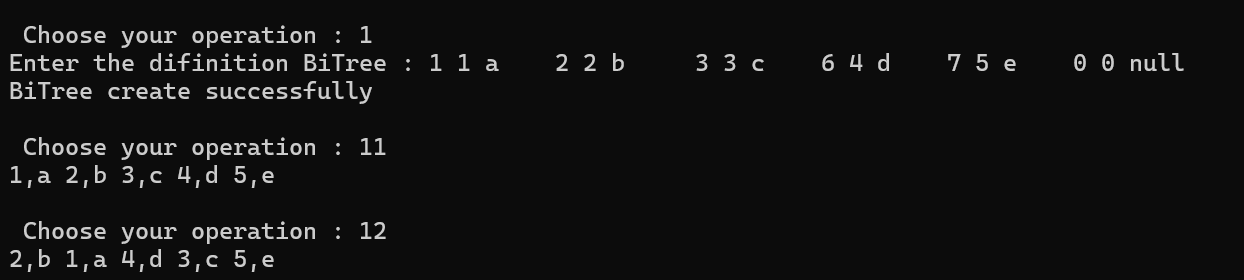
\includegraphics[width=0.6\textwidth]{images/二叉树测试1.png}
 	\caption{测试3运行结果}
 	\label{txlab}
 \end{figure}

\paragraph{ 2.}DestroyBiTree测试

测试1:在测试集1的情况下进行,测试函数能否销毁已存在的二叉树。

测试2:将测试函数能否销毁不存在的二叉树。

\vspace{0.5em}

\begin{tabular}{|c|l|c|c|c|}
	\hline
	测试编号 & 测试输入 & 预期结果 & 实际运行结果 \\
	\hline
	1 & 2 & 二叉树销毁成功! & 一致 \\
	\hline
	2 & 2 & 二叉树不存在!& 一致 \\
	\hline
\end{tabular}

~\

\begin{figure}[H]
 	\centering
 	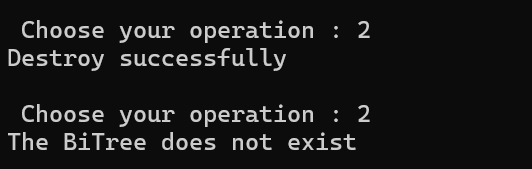
\includegraphics[width=0.6\textwidth]{images/二叉树测试2.png}
 	\caption{测试3运行结果}
 	\label{txlab}
 \end{figure}

\paragraph{ 3.}ClearBiTree测试

测试1:在测试集1的情况下进行,测试函数能否清空已存在的二叉树。

测试2:将测试函数能否清空不存在的二叉树。

\vspace{0.5em}

\begin{tabular}{|c|l|c|c|c|}
	\hline
	测试编号 & 测试输入 & 预期结果 & 实际运行结果 \\
	\hline
	1 & 3 & 二叉树清空成功! & 一致 \\
	\hline
	2 & 2$\rightarrow$3 & 二叉树不存在! & 一致 \\
	\hline
\end{tabular}

~\

\begin{figure}[H]
 	\centering
 	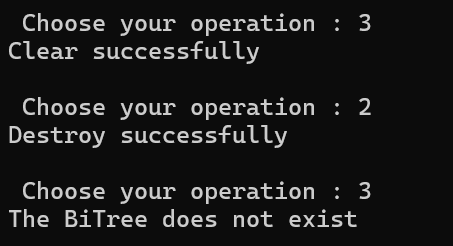
\includegraphics[width=0.6\textwidth]{images/二叉树测试3.png}
 	\caption{测试3运行结果}
 	\label{txlab}
 \end{figure}

\paragraph{ 4.}BiTreeEmpty测试

测试1:在测试集1的基础上,测试函数是否能对非空二叉树进行判空。

测试2:测试函数是否能对空二叉树进行判空。

\vspace{0.5em}

\begin{tabular}{|c|l|c|c|c|}
	\hline
	测试编号 & 测试输入 & 预期结果 & 实际运行结果 \\
	\hline
	1 & 4 & 二叉树不为空! & 一致 \\
	\hline
	2 & 2$\rightarrow$4 & 二叉树为空! & 一致 \\
	\hline
\end{tabular}

~\

\begin{figure}[H]
 	\centering
 	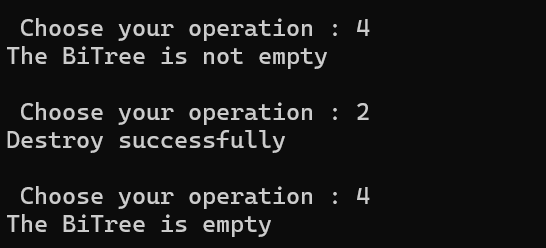
\includegraphics[width=0.6\textwidth]{images/二叉树测试4.png}
 	\caption{测试3运行结果}
 	\label{txlab}
 \end{figure}

\paragraph{ 5.}BiTreeDepth测试

测试1:测试函数能否对空二叉树求深度;

测试2:在测试集1的基础上,测试函数能否正确求得二叉树的深度。

\vspace{0.5em}

\begin{tabular}{|c|l|c|c|c|}
	\hline
	测试编号 & 测试输入 & 预期结果 & 实际运行结果 \\
	\hline
	1 & 5 & 二叉树为空! & 一致 \\
	\hline
	2 & 1$\rightarrow$5 & 该二叉树的深度为3! & 一致 \\
	\hline
\end{tabular}

~\

\begin{figure}[H]
 	\centering
 	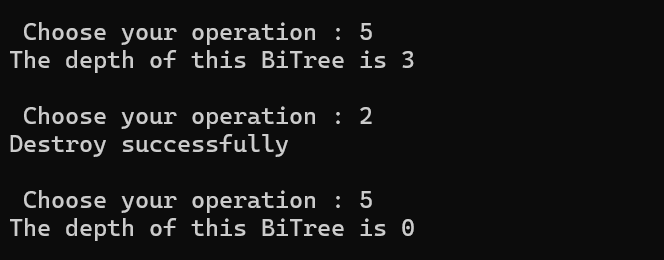
\includegraphics[width=0.6\textwidth]{images/二叉树测试5.png}
 	\caption{测试3运行结果}
 	\label{txlab}
 \end{figure}

\paragraph{ 6.}LocateNode测试 

测试1:将测试函数能否正确找到头结点并输出其值;

测试2:将测试函数能否正确找到一般结点并输出其值;

测试3:将测试函数能否正确判断结点关键字不在二叉树中。

\vspace{0.5em}

\begin{tabular}{|c|l|c|c|c|}
	\hline
	测试编号 & 测试输入 & 预期结果 & 实际运行结果 \\
	\hline
	1 & 6$\rightarrow$1 & 该节点存在!结点信息为:a & 一致 \\
	\hline
	2 & 6$\rightarrow$3 & 该节点存在!结点信息为:c & 一致 \\
	\hline
	3 & 6$\rightarrow$6 & 该节点不存在! & 一致 \\
	\hline
\end{tabular}

~\

\begin{figure}[H]
 	\centering
 	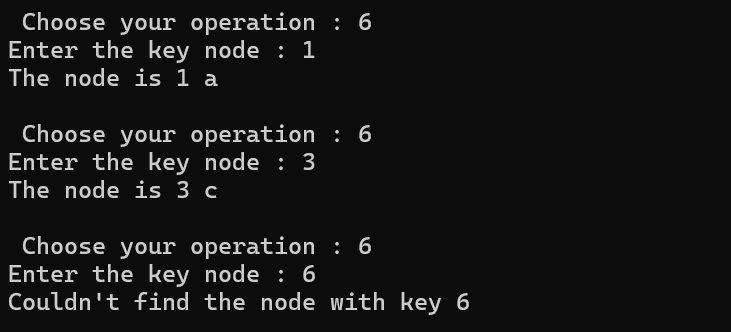
\includegraphics[width=0.6\textwidth]{images/二叉树测试6.png}
 	\caption{测试3运行结果}
 	\label{txlab}
 \end{figure}

\paragraph{ 7.}Assign测试

测试1:将测试在修改结点值时,函数能否输出正确结果(通过先序遍历结果判断);

测试2:将测试在修改结点值,但修改后关键字重复的情况下,函数能否给出判断;

测试3:将测试所修改结点不在二叉树中的情况下,函数能否给出判断。

\vspace{0.5em}

\begin{tabular}{|c|l|p{6cm}|c|}
	\hline
	测试编号 & 测试输入 & 预期结果 & 实际运行结果 \\
	\hline
	1 & 7$\rightarrow$5$\rightarrow$6 f & 结点赋值成功!

先序遍历:1,a 2,b 3,c 4,d 6,f & 一致 \\
	\hline
	2 & 7$\rightarrow$1$\rightarrow$2 g & 结点赋值失败 & 一致 \\
	\hline
	3 & 7$\rightarrow$7$\rightarrow$8 h & 结点赋值失败 & 一致 \\
	\hline
\end{tabular}

~\

\begin{figure}[H]
 	\centering
 	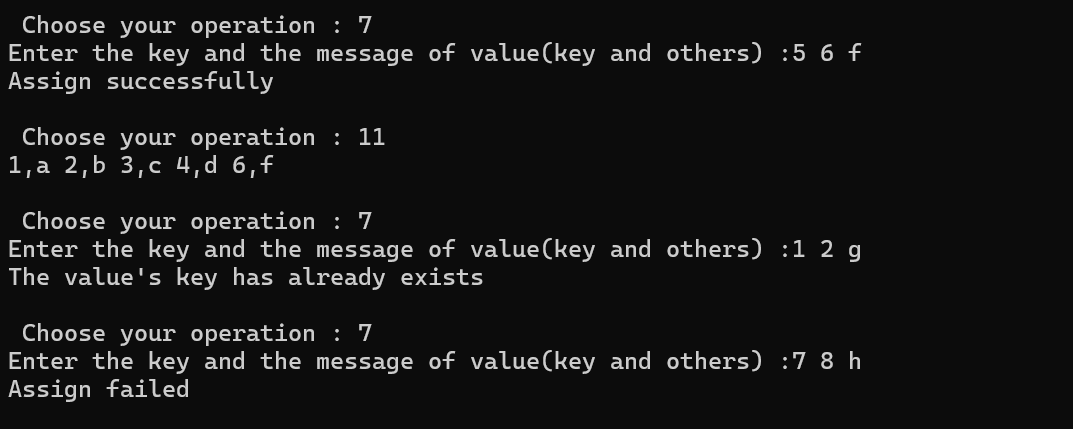
\includegraphics[width=0.6\textwidth]{images/二叉树测试7.png}
 	\caption{测试3运行结果}
 	\label{txlab}
 \end{figure}

\paragraph{ 8.}GetSibling测试

测试1,2:将输入一组互为兄弟的结点,测试函数能否输出正确结果;

测试3:将输入没有兄弟结点的结点,测试函数能否输出正确结果;

测试4:将输入一个不在二叉树中的结点,测试函数能否给出判断。

\vspace{0.5em}

\begin{tabular}{|c|l|p{7cm}|c|}
	\hline
	测试编号 & 测试输入 & 预期结果 & 实际运行结果 \\
	\hline
	1 & 8$\rightarrow$5 & 该元素兄弟结点获取成功!

该结点的兄弟结点关键字为 4 结点信息为: d & 一致 \\
	\hline
	2 & 8$\rightarrow$4 & 该元素兄弟结点获取成功!

该结点的兄弟结点关键字为 5 结点信息为: e & 一致 \\
	\hline
	3 & 8$\rightarrow$1 & 该结点不存在或不存在兄弟结点! & 一致 \\
	\hline
	4 & 8$\rightarrow$6 & 该结点不存在或不存在兄弟结点! & 一致 \\
	\hline
\end{tabular}

~\

\begin{figure}[H]
 	\centering
 	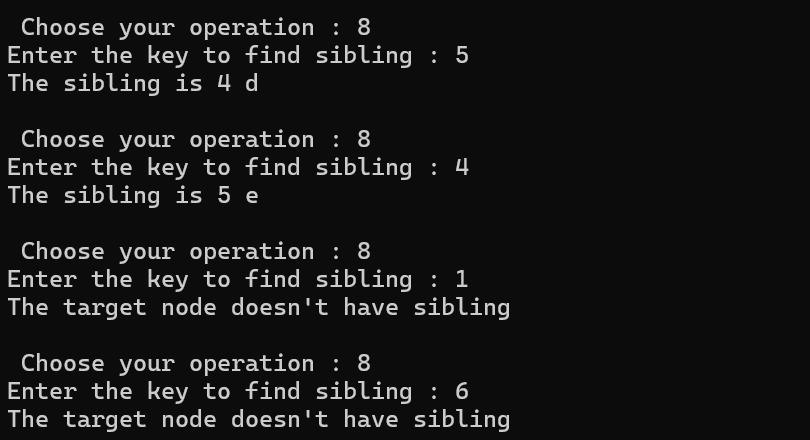
\includegraphics[width=0.6\textwidth]{images/二叉树测试8.png}
 	\caption{测试运行结果}
 	\label{txlab}
 \end{figure}

\paragraph{ 9.}InsertNode测试

输入要求:首先输入结点父亲的关键字,再输入插入要求(左孩子(0)/右孩子(1)/根节点(-1),如插入结点作为根节点,则无需考虑结点父亲的值),最后输入插入结点的值。

测试1:在测试集1的情况下进行,将新插入结点(6 f)作为根节点(-1),测试函数能否输出正确结果,通过前序遍历检验正确性;

测试2:在测试集1的情况下进行,在根节点(1 a)的左孩子插入结点(6 f),测试函数能否输出正确结果,通过前序遍历检验正确性;

测试3:在测试集1的情况下进行,在根节点(1 a)的右孩子插入结点(6 f),测试函数能否输出正确结果,通过前序遍历检验正确性;

测试4:在测试集1的情况下进行,尝试在根节点处插入一个关键字重复的结点(2 b),测试函数能否给出正确判断;

测试5:在测试集1的情况下进行,尝试插入一个结点(6 f),测试当输入的父亲结点(6)不存在于二叉树中时,函数能否给出正确的判断。

\vspace{0.5em}

\begin{tabular}{|c|l|p{6cm}|c|}
	\hline
	测试编号 & 测试输入 & 预期结果 & 实际运行结果 \\
	\hline
	1 & 9$\rightarrow$1$\rightarrow$6 f -1 & 结点插入成功!

前序遍历: 6,f 1,a 2,b 3,c 4,d 5,e & 一致 \\
	\hline
	2 & 9$\rightarrow$1$\rightarrow$6 f 0 & 结点插入成功!

前序遍历:  1,a 6,f 2,b 3,c 4,d 5,e & 一致 \\
	\hline
	3 & 9$\rightarrow$1$\rightarrow$2 b 1 & 结点插入失败(请检查该关键字是否存在或者插入关键字是否重复)! & 一致 \\
	\hline
	3 & 9$\rightarrow$6$\rightarrow$6 f 1 & 结点插入失败(请检查该关键字是否存在或者插入关键字是否重复)! & 一致 \\
	\hline
\end{tabular}

~\

\begin{figure}[H]
 	\centering
 	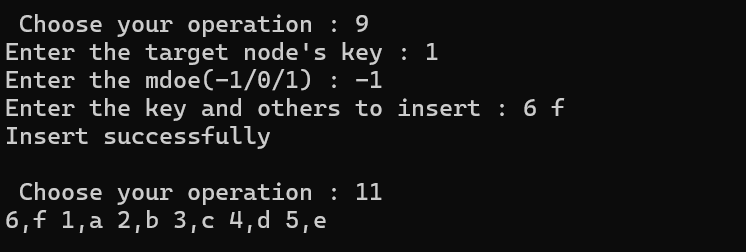
\includegraphics[width=0.6\textwidth]{images/二叉树测试9.png}
 	\caption{测试运行结果}
 	\label{txlab}
 \end{figure}

\paragraph{10.}DeleteNode测试

测试1:在测试集1的情况下进行,测试函数能否正确删除度为2的根结点,通过层序遍历的方式来检验正确性;

测试2:在测试1的基础上进行,测试函数能否正确删除度为0的叶子结点,通过层序遍历的方式来检验正确性;

测试3:在测试2的基础上进行,测试函数能否正确删除度为1的结点,通过层序遍历的方式来检验正确性。

\vspace{0.5em}

\begin{tabular}{|c|l|l|c|}
	\hline
	测试编号 & 测试输入 & 预期结果 & 实际运行结果 \\
	\hline
	1 & 10$\rightarrow$3& 结点删除成功!

层序遍历: 1,a 2,b 4,d 5,e & 一致 \\
	\hline
	2 & 10$\rightarrow$2& 结点删除成功!

层序遍历: 1,a 4,d 5,e & 一致 \\
	\hline
	3 & 10$\rightarrow$4 & 结点删除成功!

层序遍历:1,a 5,e & 一致 \\
	\hline
\end{tabular}

~\

\begin{figure}[H]
 	\centering
 	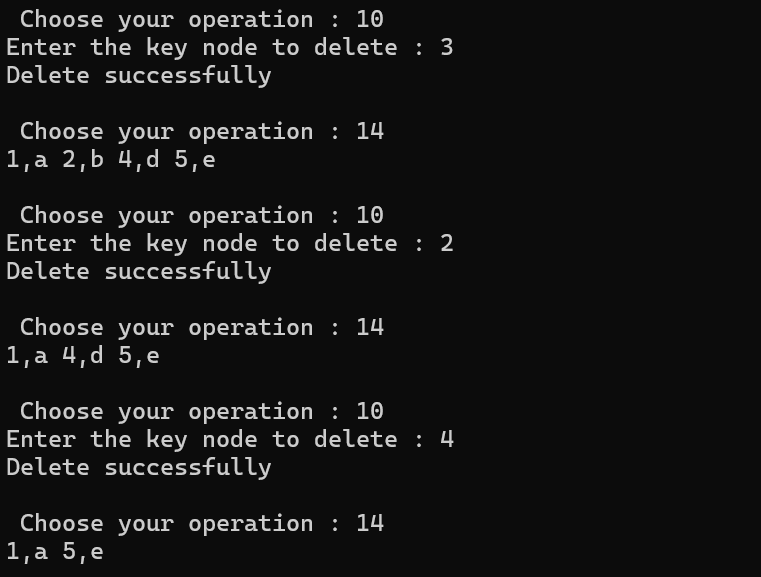
\includegraphics[width=0.6\textwidth]{images/二叉树测试10.png}
 	\caption{测试运行结果}
 	\label{txlab}
 \end{figure}

\paragraph{11.}PreOrderTraverse测试

测试1:将测试函数是否能对空树做出判断;

测试2:在测试集1的情况下进行,测试函数能否输出正确结果。

\vspace{0.5em}

\begin{tabular}{|c|p{2.7cm}|p{4.5cm}|c|}
	\hline
	测试编号 & 测试输入 & 预期结果 & 实际运行结果 \\
	\hline
	1 & 11 & 二叉树为空! & 一致 \\
	\hline
	2 & 11 & 先序遍历二叉树的结果:
 
1,a 2,b 3,c 4,d 5,e & 一致 \\
	\hline
\end{tabular}

~\

\begin{figure}[H]
 	\centering
 	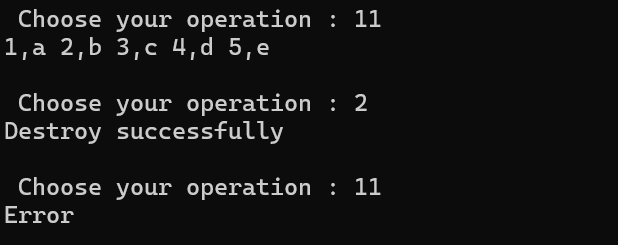
\includegraphics[width=0.6\textwidth]{images/二叉树测试11.png}
 	\caption{测试运行结果}
 	\label{txlab}
 \end{figure}

\paragraph{12.}InOrderTraverse测试

测试1:将测试函数是否能对空树做出判断;

测试2:在测试集1的情况下进行,测试函数能否输出正确结果。

\vspace{0.5em}

\begin{tabular}{|c|p{2.7cm}|p{4.5cm}|c|}
	\hline
	测试编号 & 测试输入 & 预期结果 & 实际运行结果 \\
	\hline
	1 & 12 & 二叉树为空! & 一致 \\
	\hline
	2 & 12 & 中序遍历二叉树的结果:
 
2,b 1,a 4,d 3,c 5,e & 一致 \\
	\hline
\end{tabular}

~\

\begin{figure}[H]
 	\centering
 	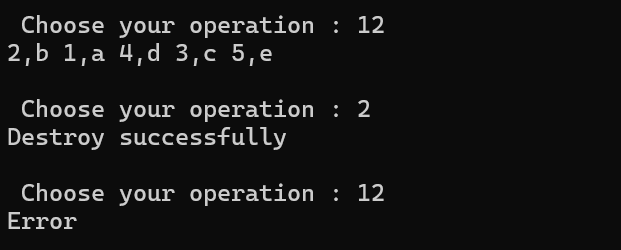
\includegraphics[width=0.6\textwidth]{images/二叉树测试12.png}
 	\caption{测试运行结果}
 	\label{txlab}
 \end{figure}

\paragraph{13.}PostOrderTraverse测试

测试1:将测试函数是否能对空树做出判断;

测试2:在测试集1的情况下进行,测试函数能否输出正确结果。

\vspace{0.5em}

\begin{tabular}{|c|p{2.7cm}|p{4.5cm}|c|}
	\hline
	测试编号 & 测试输入 & 预期结果 & 实际运行结果 \\
	\hline
	1 & 13 & 二叉树为空! & 一致 \\
	\hline
	2 & 13 & 后序遍历二叉树的结果:
 
2,b 4,d 5,e 3,c 1,a & 一致 \\
	\hline
\end{tabular}

~\

\begin{figure}[H]
 	\centering
 	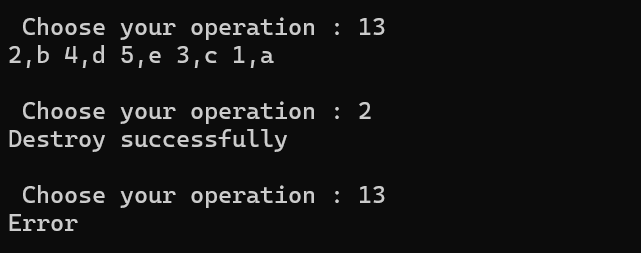
\includegraphics[width=0.6\textwidth]{images/二叉树测试13.png}
 	\caption{测试运行结果}
 	\label{txlab}
 \end{figure}

\paragraph{14.}LevelOrderTraverse测试

测试1:将测试函数是否能对空树做出判断;

测试2:在测试集1的情况下进行,测试函数能否输出正确结果。

\vspace{0.5em}

\begin{tabular}{|c|p{2.7cm}|p{4.5cm}|c|}
	\hline
	测试编号 & 测试输入 & 预期结果 & 实际运行结果 \\
	\hline
	1 & 14 & 二叉树为空! & 一致 \\
	\hline
	2 & 14 & 层序遍历二叉树的结果:

 1,a 2,b 3,c 4,d 5,e & 一致 \\
	\hline
\end{tabular}

~\

\begin{figure}[H]
 	\centering
 	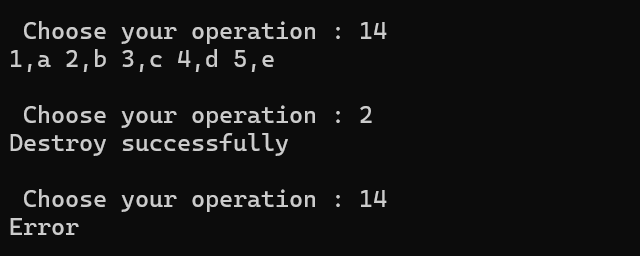
\includegraphics[width=0.6\textwidth]{images/二叉树测试14.png}
 	\caption{测试运行结果}
 	\label{txlab}
 \end{figure}

\subsubsection{附加功能测试}

\paragraph{15.}MaxPathSum测试
	
测试1:在二叉树为空的情况下进行,测试函数能否给出正确判断;

测试2:在测试集1的情况下进行,测试函数能否正常返回最大路径和。

\vspace{0.5em}

\begin{tabular}{|c|p{2.7cm}|p{6cm}|c|}
	\hline
	测试编号 & 测试输入 & 预期结果 & 实际运行结果 \\
	\hline
	1 & 15 & 二叉树为空! & 一致 \\
	\hline
	2 & 15 & 根节点到叶子结点的最大路径和为:9 & 一致 \\
	\hline
\end{tabular}

~\

\begin{figure}[H]
 	\centering
 	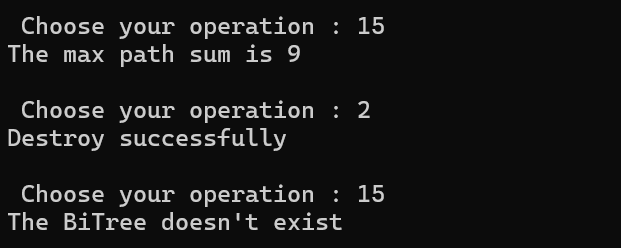
\includegraphics[width=0.6\textwidth]{images/二叉树测试15.png}
 	\caption{测试运行结果}
 	\label{txlab}
 \end{figure}

\paragraph{16.}LowestCommonAncestor测试
	
测试1:在二叉树为空的情况下进行,测试函数能否给出正确判断;

测试2:在测试集1的情况下进行,两结点均存在测试能否给出根结点;

测试3:在测试集1的情况下进行,测试第一个结点不存在时能否给出正确的判断;

测试4:在测试集1的情况下进行,测试第二个结点不存在时能否给出正确的判断。

\vspace{0.5em}

\begin{tabular}{|c|p{2.7cm}|p{6cm}|c|}
	\hline
	测试编号 & 测试输入 & 预期结果 & 实际运行结果 \\
	\hline
	1 & 16 & 二叉树为空! & 一致 \\
	\hline
	2 & 16$\rightarrow$2 4 & 两结点最近公共祖先的关键字为:1,结点信息为:a & 一致 \\
	\hline
	3 & 16$\rightarrow$6 4 & 第一个结点不存在!& 一致 \\
	\hline
	4 & 16$\rightarrow$2 6 & 第二个结点不存在! & 一致 \\
	\hline
\end{tabular}

~\

\begin{figure}[H]
 	\centering
 	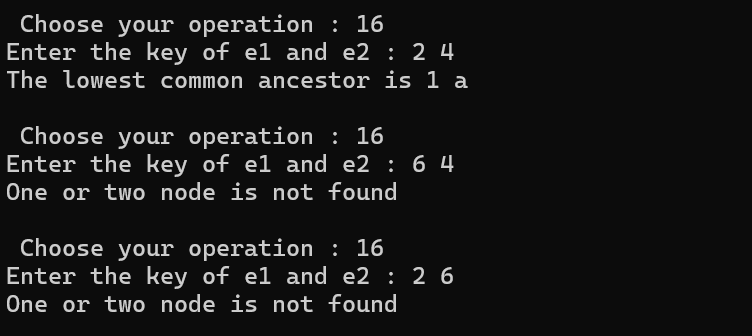
\includegraphics[width=0.6\textwidth]{images/二叉树测试16.png}
 	\caption{测试运行结果}
 	\label{txlab}
 \end{figure}

\paragraph{17.}InvertTree测试

测试1:在二叉树为空的情况下进行,测试函数能否给出正确判断;

测试2:在测试集1的情况下,测试函数能否正确反转二叉树,通过层序遍历测试函数实现正确性。

\vspace{0.5em}

\begin{tabular}{|c|p{2.7cm}|p{6cm}|c|}
	\hline
	测试编号 & 测试输入 & 预期结果 & 实际运行结果 \\
	\hline
	1 & 17 & 二叉树为空! & 一致 \\
	\hline
	2 & 17$\rightarrow$14 & 二叉树翻转成功!

层序遍历二叉树的结果:1,a 3,c 2,b 5,e 4,d & 一致 \\
	\hline
\end{tabular}

~\

\begin{figure}[H]
 	\centering
 	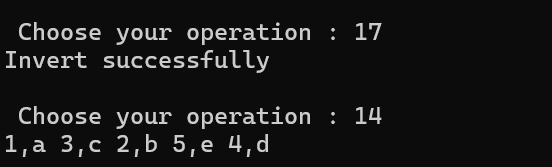
\includegraphics[width=0.6\textwidth]{images/二叉树测试17.png}
 	\caption{测试运行结果}
 	\label{txlab}
 \end{figure}

\paragraph{18.}SaveTree测试

测试1:在测试集1的情况下进行,测试函数能否正常进行写文件操作;

测试2:在文件已经有内容时,测试函数是否能够判断文件不能覆盖;

测试3:在二叉树为空的情况下进行,测试函数能否给出正确判断。

\vspace{0.5em}

\begin{tabular}{|c|p{2.7cm}|c|c|}
	\hline
	测试编号 & 测试输入 & 预期结果 & 实际运行结果 \\
	\hline
	1 & 18$\rightarrow$1.txt & 文件保存成功! & 一致 \\
	\hline
	2 & 18$\rightarrow$1.txt & 该文件已有内容,不能读入! & 一致 \\
	\hline
	3 & 2$\rightarrow$18$\rightarrow$1.txt & 二叉树不存在!文件保存失败! & 一致 \\
	\hline
\end{tabular}

~\

\paragraph{19.}LoadTree测试

测试1:在二叉树不存在的情况下进行,测试函数能否正确进行读文件操作,采用遍历二叉树的方式检验正确性。

测试2:在线性表存在的情况下进行,测试函数能否给出正确判断。

\vspace{0.5em}

\begin{tabular}{|c|p{2.7cm}|c|c|}
	\hline
	测试编号 & 测试输入 & 预期结果 & 实际运行结果 \\
	\hline
	1 & 2$\rightarrow$19$\rightarrow$1.txt & 文件录入成功! & 一致 \\
	\hline
	2 & 19$\rightarrow$1.txt & 二叉树存在!文件录入失败 & 一致 \\
	\hline
\end{tabular}

~\

\begin{figure}[H]
 	\centering
 	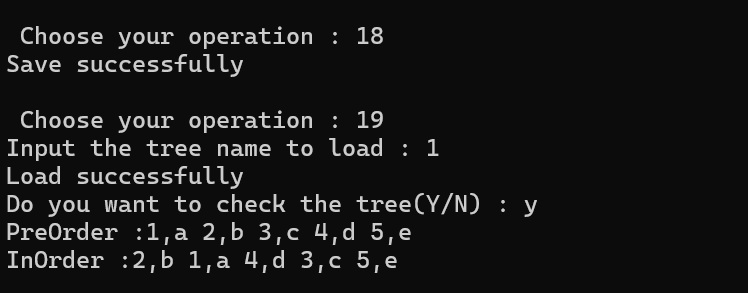
\includegraphics[width=0.6\textwidth]{images/二叉树测试18_19.png}
 	\caption{测试运行结果}
 	\label{txlab}
 \end{figure}

\paragraph{20.}AddTree测试

测试1:将测试函数能否正确添加二叉树;

测试2:在测试1的基础上进行,当二叉树名称重复时,测试函数能否给出正确的判断。

测试3:测试二叉树能否正确添加,通过遍历森林检验正确性。

\vspace{0.5em}

\begin{tabular}{|c|p{2.7cm}|c|c|}
	\hline
	测试编号 & 测试输入 & 预期结果 & 实际运行结果 \\
	\hline
	1 & 20$\rightarrow$FirstTree & FirstTree已成功添加! & 一致 \\
	\hline
	2 & 20$\rightarrow$FirstTree & 该名称的线性表已经存在! & 一致 \\
	\hline
	3 & 213& FirstTree SecondTree & 一致 \\
	\hline
\end{tabular}

~\

\begin{figure}[H]
 	\centering
 	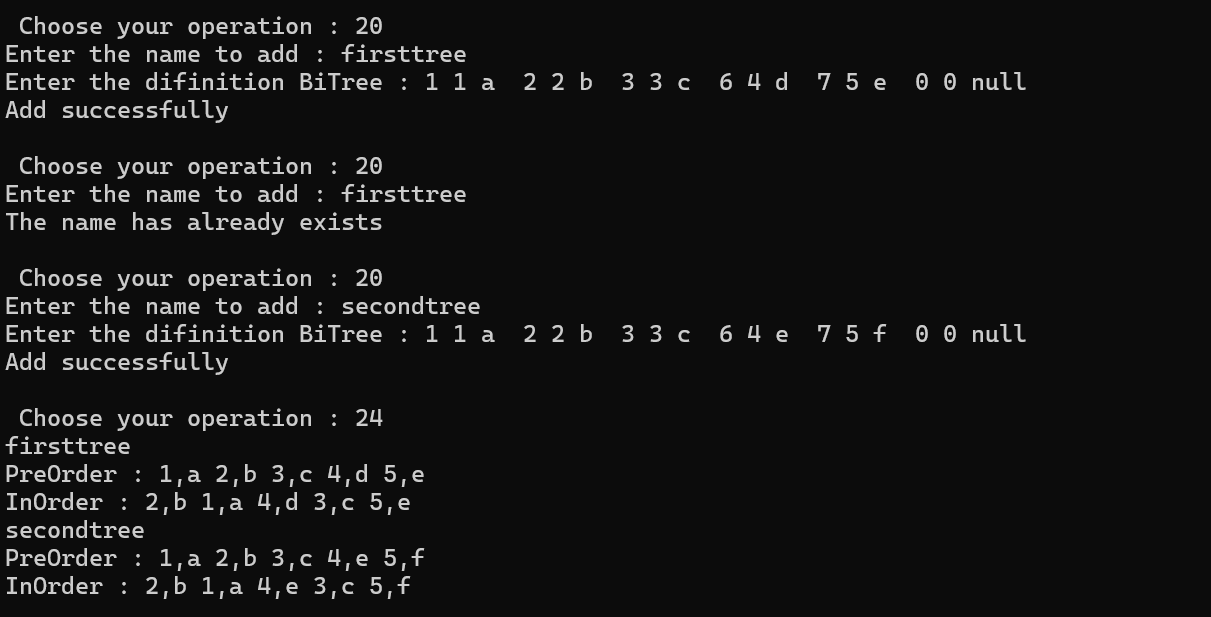
\includegraphics[width=0.6\textwidth]{images/二叉树测试20.png}
 	\caption{测试运行结果}
 	\label{txlab}
 \end{figure}

\paragraph{21.}RemoveTree测试

测试1:将测试函数能否正确销毁二叉树,采用遍历森林的方式判断正确性;

测试2:在测试集2的情况下进行,尝试销毁一个不在集合中的二叉树,测试函数能否给出正确判断。

\vspace{0.5em}

\begin{tabular}{|c|p{2.7cm}|c|c|}
	\hline
	测试编号 & 测试输入 & 预期结果 & 实际运行结果 \\
	\hline
	1 & 21$\rightarrow$FirstTree & FirstTree已成功销毁! & 一致 \\
	\hline
	2 & 21$\rightarrow$ThirdTree & 二叉树不存在! & 一致 \\
	\hline
\end{tabular}

~\

\begin{figure}[H]
 	\centering
 	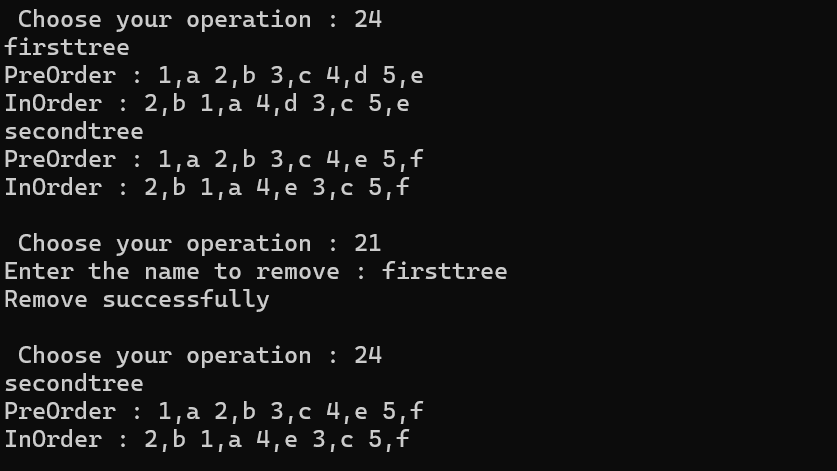
\includegraphics[width=0.6\textwidth]{images/二叉树测试21.png}
 	\caption{测试运行结果}
 	\label{txlab}
 \end{figure}

\paragraph{22.}LocateTree测试

本实验基于上个测试删除firsttree操作

测试1:将测试函数能否正确定位二叉树;

测试2:将尝试查找一个不在集合中的二叉树,测试函数能否给出正确判断。

\vspace{0.5em}

\begin{tabular}{|c|p{2.7cm}|c|c|}
	\hline
	测试编号 & 测试输入 & 预期结果 & 实际运行结果 \\
	\hline
	1 & 22$\rightarrow$SecondTree & 该二叉树的逻辑索引为:1 & 一致 \\
	\hline
	2 & 22$\rightarrow$FirstTree & 二叉树查找失败! & 一致 \\
	\hline
\end{tabular}

~\

\begin{figure}[H]
 	\centering
 	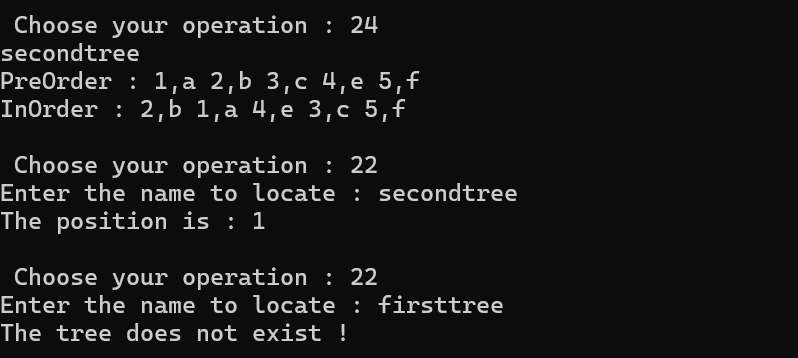
\includegraphics[width=0.6\textwidth]{images/二叉树测试22.png}
 	\caption{测试运行结果}
 	\label{txlab}
 \end{figure}

\paragraph{23.}SwitchTrees测试
	
测试1:测试函数能否正确判断非法的名称;

测试2:测试函数能否正确地实现选取线性表操作。

\vspace{0.5em}

\begin{tabular}{|c|p{2.7cm}|c|c|}
	\hline
	测试编号 & 测试输入 & 预期结果 & 实际运行结果 \\
	\hline
	1 & 24$\rightarrow$thirdtree & 二叉树切换失败! & 一致 \\
	\hline
	2 & 24$\rightarrow$firsttree & 二叉树切换成功! & 一致 \\
	\hline
\end{tabular}

~\

\begin{figure}[H]
 	\centering
 	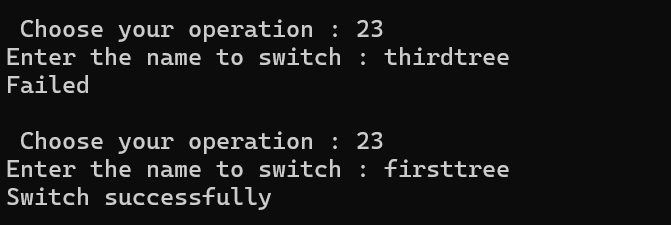
\includegraphics[width=0.6\textwidth]{images/二叉树测试23.png}
 	\caption{测试运行结果}
 	\label{txlab}
 \end{figure}

\paragraph{23.}ShowAllTrees测试
	
测试1:测试函数能否正确遍历各个线性表;

\vspace{0.5em}

\begin{tabular}{|c|p{2.7cm}|c|c|}
	\hline
	测试编号 & 测试输入 & 预期结果 & 实际运行结果 \\
	\hline
	1 & 23 & FirstList SecondList & 一致 \\
	\hline
\end{tabular}

~\

\begin{figure}[H]
 	\centering
 	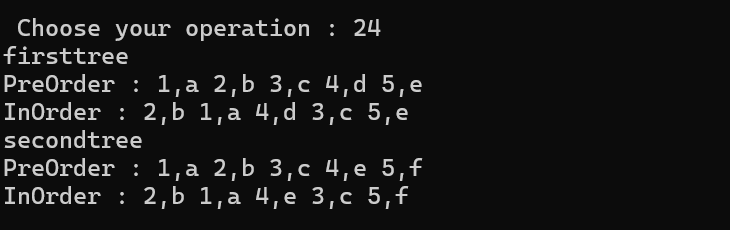
\includegraphics[width=0.6\textwidth]{images/二叉树测试24.png}
 	\caption{测试运行结果}
 	\label{txlab}
 \end{figure}

测试小结

24个函数基本符合了测试要求,在正常和异常用例的条件下均可以正常运行。需要注意的是,在对某些函数进行测试时,出于篇幅限制,没有测试二叉树不存在的情况,同时对于附加功能函数没有具体给测试后的控制台界面。

\subsection{实验小结}

这次实验使用链式存储结构实现二叉树,让我更加清楚了二叉树的物理结构、数据结构类型、基本操作及实现。认识到二叉树的存储结构与线性存储结构的不同。这次实验中使用顺序表来管理多树(森林),提高了本次实验的程序的功能性。

在本次实验过程中,多个函数使用递归调用自身的形式编写函数,同时通过设置全局变量的方式解决递归过程中变量的初始化和迭代问题。

除此以外,在用非递归方式实现遍历时,使用了栈的存储结构和相应操作,在实现层序遍历时,使用了队列的存储结构和相应操作。通过不同数据结构的运用,使得问题的解决更加便利。

同时,基于二叉链表的二叉树的实验的难度较前两次都有所提升,极大地提升了我的编程水平。

本次实验使我加深了对二叉树的概念、基本运算的理解,掌握了二叉树的基本运算的实现。熟练了二叉树的逻辑结构和物理结构的关系。在今后的学习过程当中应该更多地从数据结构的角度去分析如何进行数据的存储、读取和处理,以达到更简便地解决实际问题的目的。


\newpage

\section{课程的收获和建议}

通过本学期的数据结构实验课,我收获了很多知识,非常感谢老师和助教的帮助,同时包括我自己的努力,让我在数据结构方面收获很多,编程能力和思维能力有了很大的提高。

\subsection{基于顺序存储结构的线性表实现}

通过实验达到:(1)加深对线性表的概念、基本运算的理解;(2)熟练掌握线性表的逻辑结构与物理结构的关系;(3)物理结构采用顺序表,熟练掌握顺序表基本运算的实现。在实验过程中,对于线性表的本质有了更加深入的思考与理解,提升了思维能力。

\subsection{基于链式存储结构的线性表实现}

通过实验达到:(1)加深对线性表的概念、基本运算的理解;(2)熟练掌握线性表的逻辑结构与物理结构的关系;(3)物理结构采用单链表,熟练掌握线性表的基本运算的实现。在实验过程中,清晰了顺序存储结构和单链表存储结构之间的区别与联系,对于线性表有了深刻的体会,同时能够灵活应用。

\subsection{基于二叉链表的二叉树实现}

通过实验达到:(1)加深对二叉树的概念、基本运算的理解;(2)熟练掌握二叉树的逻辑结构与物理结构的关系;(3)以二叉链表作为物理结构,熟练掌握二叉树基本运算的实现。在实验过程中,对于二叉树特殊的存储结构能够很好地应用,同时对于递归操作有了更加深刻的理解。

\subsection{基于邻接表的图实现}

通过实验达到:(1)加深对图的概念、基本运算的理解;(2)熟练掌握图的逻辑结构与物理结构的关系;(3)以邻接表作为物理结构,熟练掌握图基本运算的实现。在实验过程中,学会使用图的邻接表创建无向图,同时由于图的复杂性,对于心理素质的锻炼起到了很大的效果。

\addcontentsline{toc}{section}{参考文献}
\nocite{*} %% 作用是不对文献进行引用,但可以生成文献列表
\bibliographystyle{HustGraduPaper}
\begin{thebibliography}{}
\bibitem[]{1}严蔚敏等.数据结构(C语言版).清华大学出版社
\bibitem[] {2}Larry Nyhoff. ADTs, Data Structures, and Problem Solving with C++.  Second Edition,Calvin College,2005
\bibitem[] {3}殷立峰. Qt C++跨平台图形界面程序设计基础. 清华大学出版社,2014:192~197
\bibitem[] {4}严蔚敏等.数据结构题集(C语言版).清华大学出版社
\end{thebibliography}

\section{附录A 基于顺序存储结构线性表实现的源程序}

\begin{lstlisting}[language=c]

\end{lstlisting}

\newpage
\section{附录B 基于链式存储结构线性表实现的源程序}

\begin{lstlisting}[language=c]

\end{lstlisting}

\newpage
\section{附录C 基于二叉链表二叉树实现的源程序}

\begin{lstlisting}[language=c]

\end{lstlisting}

\newpage
\section{附录D 基于邻接表图实现的源程序}
\begin{lstlisting}[language=c]

\end{lstlisting}
\end{document}